\chapter{慢性腹痛}

慢性腹痛是指起病缓慢、病程长,或急性发病后反复发作的腹痛。慢性腹痛是一个常见的症状,原因相当复杂,往往引起诊断上的困难。同时慢性腹痛与急性腹痛的病因,又往往互相交叉,故在诊断时应相互参考。有些慢性腹痛有一定的规律和特点,对鉴别诊断可有帮助。

临床上对于慢性腹痛病例的诊断与鉴别诊断,首先可参考下列几方面的临床表现:

\section{(一)既往史}

患者既往的急性阑尾炎、急性胆囊炎、急性胰腺炎、腹部手术等病史,对提供慢性腹痛的病因诊断有帮助,但仍须注意有无慢性腹痛的其他原因并存。

\section{(二)腹痛的部位}

慢性腹痛患者就诊时通常能明确指出腹痛的部位,这对病变的定位有一定的意义。

\section{(三)腹痛的性质}

溃疡病多呈节律性周期性中上腹痛,部分有季节性;肝癌的疼痛常呈进行性加剧;肠寄生虫病多为发作性隐痛或绞痛,常可自行缓解;结肠、直肠疾病常为阵发性痉挛性腹痛,排便后疼痛常可缓解。直肠炎也常伴有里急后重。

\section{(四)腹痛与体位关系}

胃黏膜脱垂症患者左侧卧位常可使疼痛减轻或缓解,而右侧卧位则可使疼痛加剧;在胃下垂、肾下垂与游走肾患者,站立过久及运动后疼痛出现或加剧,仰卧或垫高髋部仰卧时减轻或消失;胰体部痛患者仰卧时疼痛加剧,在前倾坐位或俯卧位时减轻;膈疝患者的上腹痛在食后卧位时出现,而在站立位时缓解;良性十二指肠梗阻或胰体癌时上腹胀痛可于俯卧位时缓解。

\section{(五)腹痛与其他症状的关系}

1.慢性腹痛伴有发热提示有炎症、脓肿或恶性肿瘤的可能性。

2.慢性腹痛伴有呕吐胃内容物,伴有宿食,伴或不伴胆汁,常见于胃十二指肠的梗阻性病变,如消化性溃疡病合并梗阻、胃黏膜脱垂症、胃癌、十二指肠壅积症、胰腺肿瘤等。反射性呕吐可见于慢性胆道疾病、慢性盆腔疾病等。

3.慢性腹痛伴有腹泻多见于肠道慢性炎症,也可见于慢性肝脏与胰腺疾病。

4.慢性腹痛伴有脓血便者应多考虑慢性感染性肠炎(如慢性痢疾等)与慢性非特异性肠炎(如溃疡性结肠炎等);便血者应注意肠肿瘤、肠结核、炎症性肠病等。

5.慢性腹痛伴有包块应注意鉴别炎症性包块、肿瘤、胃黏膜脱垂症、痉挛性结肠、慢性脏器扭转等疾病。

根据慢性腹痛的部位与特点,结合有关的病史、体征、实验室检查与器械检查,如大便常规、胃液分析、十二指肠引流液、血清生化学检查和B超检查、各种方式的X线检查、电子胃镜与结肠镜、胶囊内镜、双气囊小肠镜、电子计算机X线体层扫描(CT)、磁共振(MRI)、正电子发射体层扫描(PET)检查等,必要实行腹腔镜或剖腹探查,进行全面分析,对疑难慢性腹痛患者可作出正确的诊断。

有些慢性腹痛疾病,在内科临床上不能解决诊疗问题时,应商请其他有关的临床专科医生共同研究处理。

从临床实际出发,本文对慢性腹痛病例的讨论,按表\ref{tab26-1}的8个腹部分区(参见图\ref{fig25-1})进行。这种分区仍存在缺点,不少疾病的疼痛可不只在一个部位出现,甚至可变换部位;为了避免叙述重复,根据该病最常出现疼痛的位置,纳入相应的腹部分区进行讨论。

\begin{longtable}{c}
 \caption{慢性腹痛疾病的分类}
 \label{tab26-1}
 \endfirsthead
 \caption[]{慢性腹痛疾病的分类}
 \endhead
 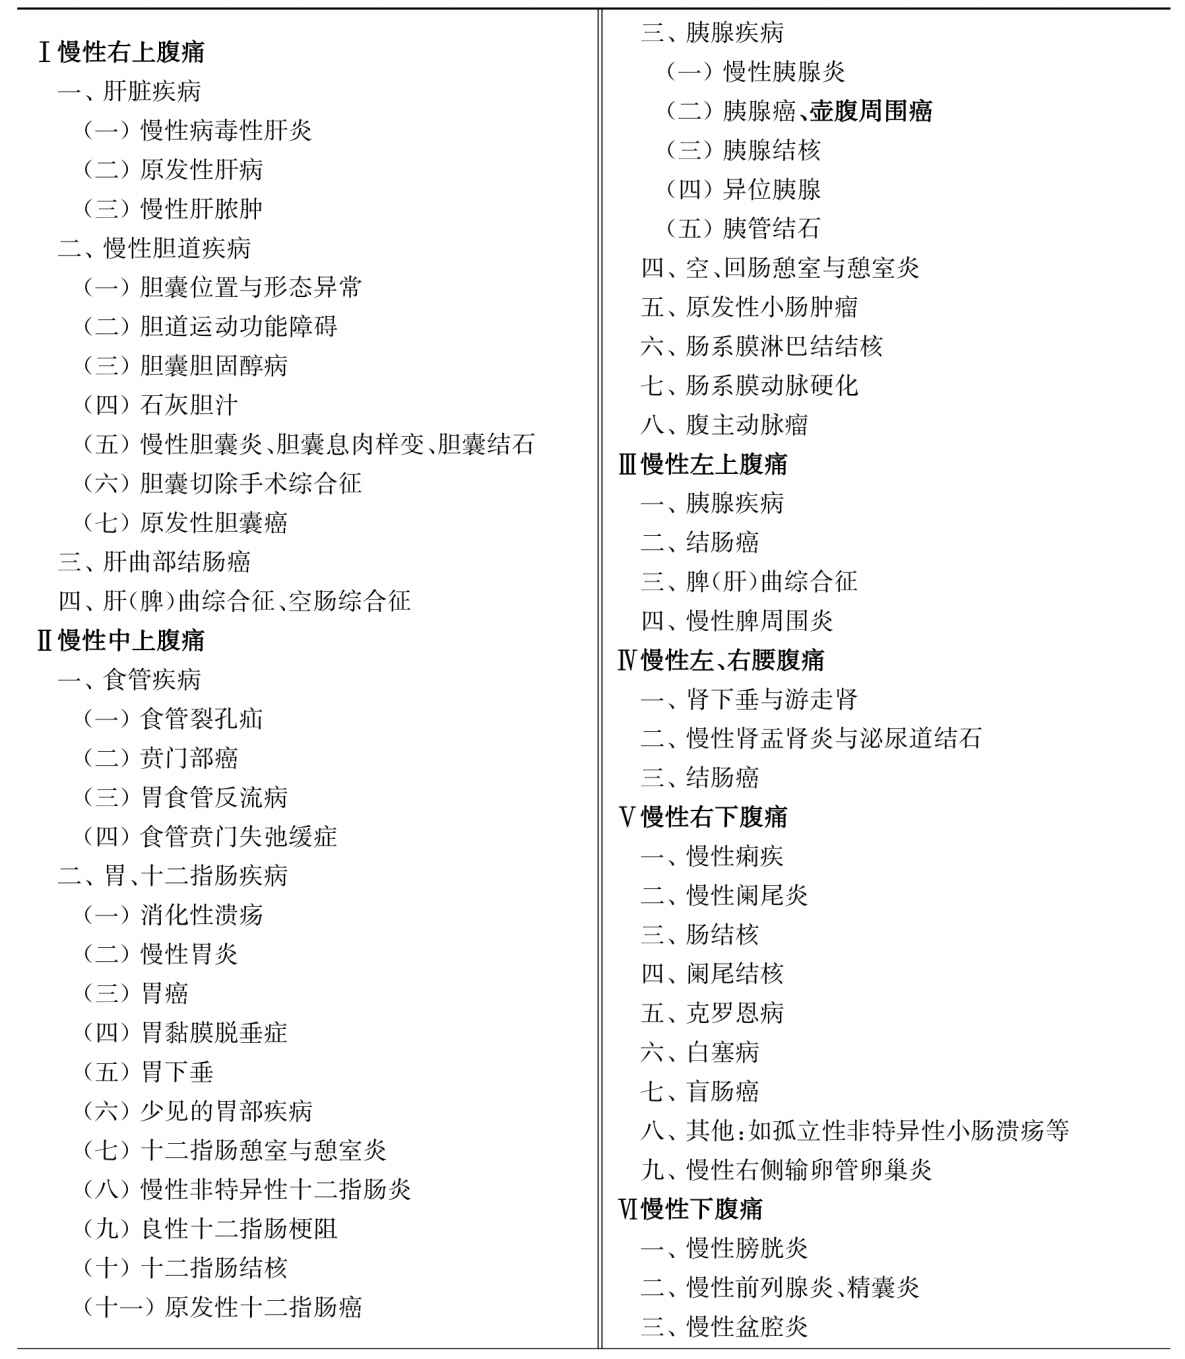
\includegraphics[width=\textwidth,height=\textheight,keepaspectratio]{./images/Image00147.jpg}\\
 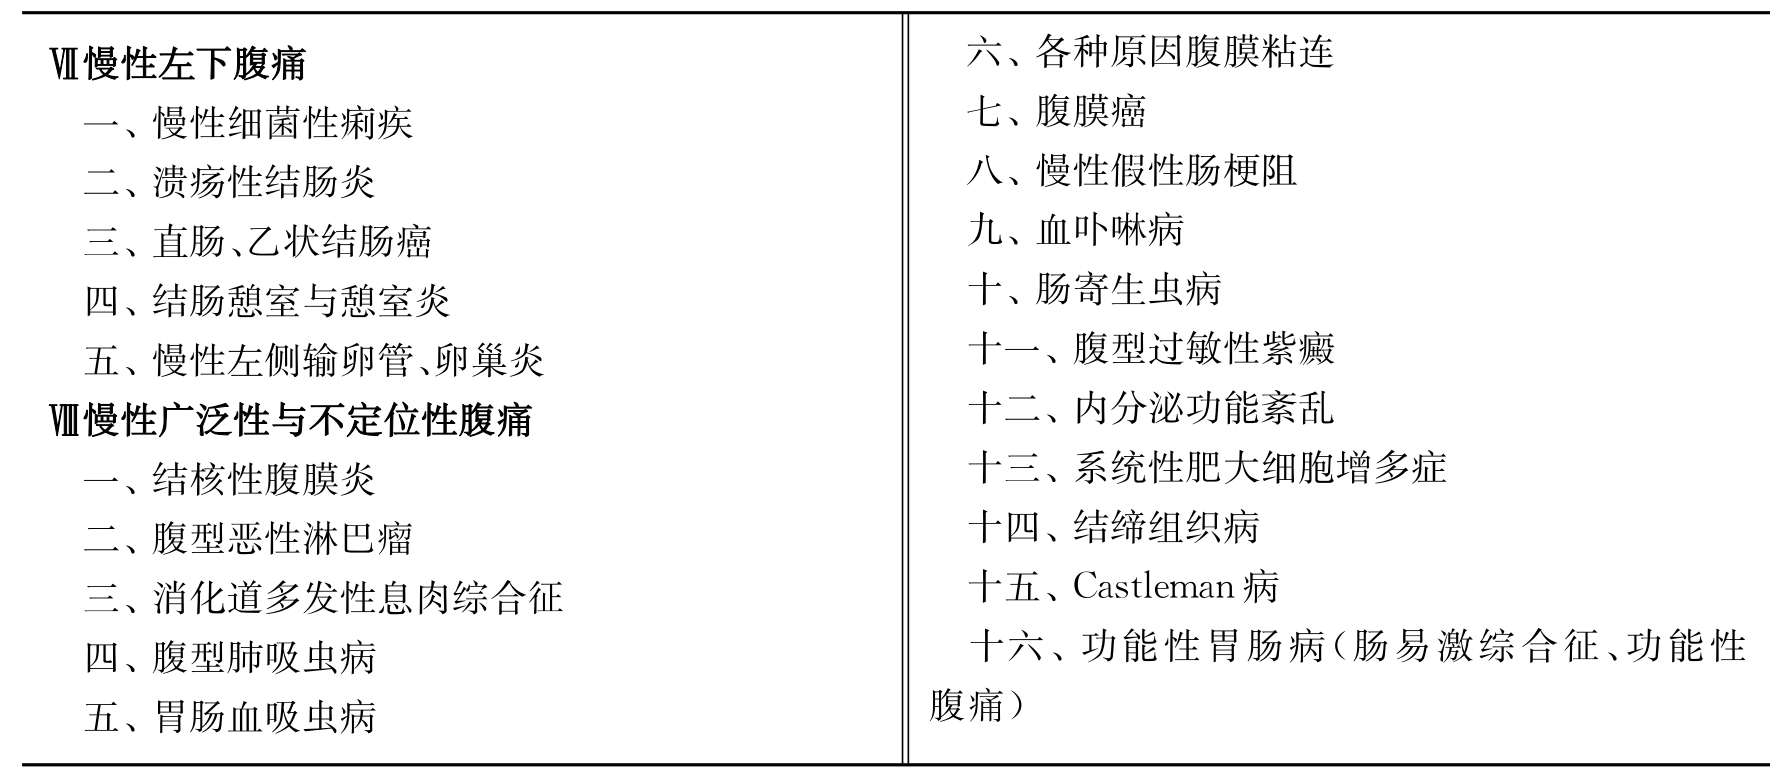
\includegraphics[width=\textwidth,height=\textheight,keepaspectratio]{./images/Image00148.jpg}
 \end{longtable}

\protect\hypertarget{text00203.html}{}{}

\section{80 慢性右上腹痛}

\subsection{80.1 肝脏疾病}

\subsubsection{一、慢性病毒性肝炎}

在慢性病毒性肝炎时可出现有上腹持续性隐痛,偶尔也可为相当剧烈的阵发性痛,这是由于肝包膜牵张、肝脏周围炎或胆道痉挛所致。慢性病毒性肝炎可与慢性肝胆道感染相混淆。慢性病毒性肝炎误诊为慢性肝胆道感染者甚少,而慢性肝胆道感染误诊为慢性病毒性肝炎者则有之。有时两者也可并存。慢性病毒性肝炎疼痛与慢性胆囊炎疼痛的鉴别是:前者疼痛与进食关系不明显,常伴有肝区压痛;后者疼痛常于进食油腻饮食后诱发或加重,胆囊区压痛明显,Murphy征阳性,必要时借助血清酶学和影像学检查结果进一步鉴别。此外尚须与肝脓肿、肝癌等相鉴别。

肝炎后综合征少数急性病毒性肝炎在恢复期之后仍有食欲减退、疲乏、腹部不适及其他胃肠道症状。肝炎后综合征就是指这种状态,是由急性病毒性肝炎衍变而来。常见的肝脏疾病肝功能检查和肝穿刺活检都无异常改变,影像学检查正常,一般认为患者的症状和精神体质因素有关。但是,有些活动性肝脏病也可无肝功能检查的异常,因此,如无正常的肝活检结果或较长时期的随诊,则不应草率作出肝炎后综合征的诊断。

\subsubsection{二、原发性肝癌}

原发性肝癌患者常有右上腹痛,但此时大多能触及大而硬的肝脏。由于在肝硬化基础上发生肝癌的发病率较高,因此肝硬化患者在短期内出现肝大与肝区疼痛时,须注意肝癌的可能性,病毒性肝炎或肝硬化病史,血清甲胎蛋白水平增高,B超、CT、MRI、PET及肝动脉造影及肝活检等有助于明确诊断。引起腹痛的原因主要是肝包膜过度牵张、肝脏周围炎、癌组织侵及腹膜或膈所致,肝癌患者出现肝区疼痛突然加剧,尤其是同时伴有发热应考虑肝癌破裂出血或缺血坏死的可能。肝癌在夜间或劳动后往往加剧,在诊断上易与肝脓肿或胆囊炎混淆。肝癌的疼痛是进行性加剧,肝呈进行性增大、质硬,表面凹凸不平,而肝脓肿与胆囊炎则无此征象。

\subsubsection{三、慢性肝脓肿}

慢性肝脓肿常呈右上腹持续性胀痛,肝大,局限性压痛比较明显,常伴有发热、消瘦等全身感染性症状,须注意与原发性肝癌相鉴别(参见第106.2节)。

\subsection{80.2 慢性胆道疾病}

慢性胆道疾病临床上常见,主要症状是反复发作的、不同程度的右上腹绞痛,病因多由于结石,而有些由于寄生虫(华支睾吸虫、蛔虫、梨形鞭毛虫)或功能性。此病的临床表现与慢性胃十二指肠疾病(如消化性溃疡、慢性胃炎等)、慢性胰腺疾病、肝(脾)曲综合征等有时相似,病程迁延,常有再发。B超和CT、MRCP、ERCP、PTC等已应用于胆道疾病的诊断,可取代许多其他的检查(如十二指肠引流液的检查等)。

慢性胆道疾病可区分为器质性与功能性两类,而以前者为多。单纯功能性的少见。据国外文献报道,慢性胆道功能障碍往往也有器质性因素为背景。

\subsubsection{一、胆囊位置与形态的异常}

胆囊位置的常态变异一般无多大临床意义。瘦长体型者的胆囊呈悬垂位,而肥胖体型者的胆囊呈横置位。如位置异常影响胆囊排空功能,或并发胆囊周围炎症性粘连,则可引起临床症状。悬垂型胆囊如为钟摆样,则可引起胆囊扭转或排空障碍而出现症状。患者大都是肌肉薄弱的瘦长体型的人。

胆囊形态异常有下列几种:胆囊基底部卷缩、胆囊中隔形成、葫芦形狭窄及憩室形成等。如形态异常发生于胆囊漏斗部、囊颈部或胆囊管,常有临床意义。

胆囊虹吸病胆囊漏斗部、囊颈部和胆囊管首段等三部分组成胆囊虹吸,由于它的管径小而弯,漏斗部与囊颈部、囊颈部与胆囊管之间各有瓣膜和括约肌,在解剖上是一个薄弱的部分,故当有炎性肿胀、纤维性硬化和增厚、瓣膜畸形、腹膜被覆异常,以及外部压迫等因素影响时,均可引起虹吸通路狭窄而发生胆囊虹吸病,出现胆囊运动功能障碍和胆绞痛。此病的主要诊断根据是:①反复发作的胆绞痛;②油腻饮食(包括胆囊造影的脂肪餐)可激发胆绞痛发作;③十二指肠引流时,B液胆汁量少,流出时间延长,流时作痛;④胆道造影显示胆总管正常,胆囊充盈饱满、张力强、收缩力大,漏斗部或囊颈扩张;⑤胆囊排空延缓;⑥患者无引起胆道运动功能障碍的十二指肠球后溃疡、胆道结石、慢性胰腺炎、慢性结肠炎、胆道华支睾吸虫感染等疾病。

\subsubsection{二、胆道运动功能障碍}

真正的胆道运动功能障碍是单纯的功能性排空障碍,而并非器质性病变。胆道运动功能障碍是少见的疾病,主要有下列两种临床类型:

\paragraph{(一)内分泌失调型}

此型是最常见的胆道运动功能障碍,发生于年轻妇女;典型的发作在月经前期,伴有雌激素过多的症状(乳房胀痛、盆腔部沉重感)。患者主诉右上腹部或上腹部疼痛,或向肩胛部放射。无发热与黄疸,但常有呕吐。体检发现胆囊触痛征阳性。症状的发生可与饮食有关,也可与饮食无关;情绪激动常为诱发因素。在月经前隔天肌注黄体酮10mg,连续数次,常有较好疗效。

\paragraph{(二)伴有偏头痛的胆道运动功能障碍}

在此型病例中,2/3的患者在长期罹患偏头痛之后发生胆道症状,1/3病例偏头痛与胆道症状同时出现。发病机制认为一方面由于血管舒缩中枢功能障碍,另一方面由于胆汁分泌的异常增多。后者乃因偏头痛发作时肝血流量高度增加所致,注射酒石酸麦角胺后则能抑制之。胆汁分泌的异常增多,而同时胆道口括约肌发生痉挛,易引起胆总管扩张。伴有偏头痛的胆石症患者,胆囊切除后大多数仍有偏头痛发作,且常因胆道口括约肌运动障碍而同时发生胆道痉挛性疼痛。

胆道运动功能障碍的诊断须细心排除器质性胆囊与胆管疾病、肝脏病、邻近器官(肾、胰、胃十二指肠)的疾病、膈疝、亚急性阑尾炎、结肠炎、结肠癌、结肠激惹综合征等疾病而确定之。静脉胆囊造影对诊断帮助甚大,因可使胆总管一并显影。在发作缓解期进行胆囊造影,其显影与排空均正常,胆总管充盈正常;而发作期胆囊排空困难或延迟,或胆总管异常扩张(由于胆道口括约肌痉挛引起),则甚有诊断价值。

胆道口括约肌痉挛可反射性由腹腔内各脏器的慢性炎症而引起,如慢性阑尾炎、慢性附件炎等。曾报告患者有典型的症状(右上腹痛、恶心、不耐受脂肪等),而静脉胆道X线造影无发现,经切除阑尾后症状消失。

\subsubsection{三、胆囊胆固醇病}

胆囊胆固醇病是一种胆囊代谢障碍疾病,发病机制多数认为是由于胆囊黏膜吸收胆固醇过多所致。临床表现可为消化不良症状,也可引起胆绞痛。胆囊胆固醇病可引起胆囊淤滞与发炎,故常为胆囊结石的前期。中年或中年以上、身体肥胖的患者,如有胆囊病征象,而过去无胆囊炎发作史,血清胆固醇增高,X线检查无胆结石发现,应考虑胆囊胆固醇病的可能性。此病往往须经手术方能确诊。

\subsubsection{四、石灰胆汁}

石灰胆汁是十分少见的疾病,发病机制尚未十分明了,国内仅有少数病例报告。石灰胆汁主要由碳酸钙及磷酸钙组成。临床表现与慢性胆囊炎相似。患者常有右上腹隐痛、厌油腻、食欲减退等症状,有时伴有恶心、呕吐。少数病例可无症状。X线平片检查有特异性表现,胆囊的影像极似造影时显影的胆囊,如胆囊同时有透放射线的结石存在时,常被石灰胆汁所衬托而清楚地显出。

\subsubsection{五、慢性胆囊炎}

慢性胆囊炎无典型症状。患者可能有持续性右上腹钝痛或不适感、胃灼热感、腹胀、嗳酸、嗳气、恶心等症状,有时可出现右肩胛区疼痛。患者如无急性发作,每难于诊断,临床上常易误诊为溃疡病、慢性胃炎、胃消化不良,甚至被诊为慢性病毒性肝炎或神经症。患者进食油腻饮食后往往恶心、疼痛加剧,此点与消化性溃疡病及慢性胃炎不同。体检可发现以下压痛点:①胆囊压痛点,即Murphy点,在右侧腹直肌外缘与肋弓的交点;②第8~10胸椎右旁压痛点;③右膈神经压痛点(在颈部右侧胸锁乳突肌两下脚之间),此压痛点尤有诊断意义。炎症发作时胆囊触痛征阳性。影像学诊断首选B超扫描。而十二指肠引流、腹部平片及胆囊造影等对慢性胆囊炎的诊断也有重要意义。十二指肠引流时,如B液胆汁中黏液增多,大量白细胞(特别是被胆汁染黄的白细胞),胆汁细菌培养有致病菌,则可诊断为胆囊炎。有时虽然白细胞不多,而多次B液胆汁培养某种致病性细菌持续阳性,或A、B、C液胆汁中培养出的细菌一致,也可肯定诊断。如仅有白细胞或细菌培养菌种变换不定,则属可疑,须反复引流以澄清诊断。胆汁中细菌以大肠杆菌为最常见,有时也可发现梨形鞭毛虫、华支睾虫卵、阿米巴等。十二指肠引流检查对临床不典型胆道感染和泥沙样结石有一定诊断意义,胆道X线检查阴性病例十二指肠引流可为阳性。但阳性率和检查次数与病程早晚有关,病程愈早和引流检查次数愈多,阳性率愈高。胆囊造影对慢性胆囊炎的诊断价值甚大,可发现透X线的胆石,胆囊肿大、缩小或变形,胆囊收缩功能不良,胆囊显影淡薄或不显影等征象。最有诊断价值的是发现胆石的存在。如患者无肝功能损害或胆红素代谢功能失常(如Dubin-Johnson综合征),而静脉胆囊造影不显影,甚至增大造影剂剂量时也不显影,对诊断慢性胆囊炎甚有价值。如胆囊不显影是由于肝功能损害,在造影前数天加强护肝饮食(基本原则是低脂肪、适量蛋白质、高糖)及护肝药物治疗,以改善肝功能,可使胆囊显影率提高。临床上一部分病例虽有明显的慢性胆囊炎症状,而X线胆囊造影却显示正常,十二指肠引流也正常。对这些病例,须考虑慢性胃十二指肠疾病、微小的胆石或胆囊胆固醇病、结肠肝曲综合征、胆道口括约肌的痉挛或纤维化等情况。后者可经由电子十二指肠镜作胆道逆行造影术(ERCP)以明确诊断。

胆囊息肉样变是胆囊黏膜局限性隆起病变的总称。绝大多数为良性,只少数为恶性。本病无特异临床表现,症状类似慢性胆囊炎或胆石症。约1/5患者无症状。B超是首选的诊断方法,检出率达89.0\%,特异性高达92.8\%。年龄大于50岁或合并胆囊结石者高度警惕恶性变的可能性。

胆囊腺肌增生病少见。本病是一种良性胆囊疾病,患者常有右上腹痛、发热,可出现黄疸,临床表现类似慢性胆囊炎。B超扫描可误认为恶性肿瘤,最后经手术探查而确诊。

梨形鞭毛虫性胆道感染少见,大多呈慢性经过,临床表现如同慢性细菌性胆囊炎,诊断主要依靠十二指肠引流胆汁检查。本病也可引起急性胆道炎症状。甲硝唑治疗疗效良好。

胆囊结石约70\%胆囊炎病例有之。胆囊结石的症状颇不一致。患者可有上腹或右上腹闷胀,或其他消化不良症状。体检可无特别体征,如并发胆囊炎则胆囊部位出现压痛。B超扫描对检测胆囊结石帮助较大,不少无症状结石可被检出,还可能预测胆石的成分与结构。腹部平片可见到不透X线的结石阴影。

\subsubsection{六、胆囊切除术后综合征}

胆囊切除术后综合征(post cholecystectomy
syndrome,PCS)是指胆囊切除术后原有的症状没有消失,或在此基础上又有新的症状发生的一组症候群,包括轻度非特异性的消化道症状(上腹闷胀不适、腹痛、肩背部疼痛不适、消化不良、食欲减退、恶心或伴呕吐、嗳气、大便次数增多等)和特异性的胆道症状(右上腹剧痛、胆绞痛、发热、黄疸等)。PCS又有广义及狭义之分,广义上的PCS是指各种原因所致,包括胆系和胆系以外器质性病变以及无器质性原因的PCS;狭义上,PCS仅指目前检查手段不能发现胆系内外有器质性病变而临床症状又持续存在的非器质性PCS。PCS的发病率约10\%~30\%,多于胆囊切除术后数周或数月内发生,女性多于男性,症状可由精神刺激、酒精、进油腻性食物等因素所诱发。多数PCS患者症状比较轻,但部分病例诊断较困难,且治疗较为棘手。PCS的病因包括胆系原因、胆系外原因以及非胆系内外原因。胆系原因包括胆囊管留置过长及残余胆囊,胆总管结石与损伤、胆道解剖变异及其他胆道疾病、Oddi括约肌功能障碍和十二指肠乳头憩室及乳头旁憩室;非胆系内外原因主要是指肠易激综合征、胃食管反流性疾病、消化不良、冠心病、食管裂孔疝、溃疡病、胰腺炎症及肿瘤、胃肠道肿瘤、阑尾炎、慢性肠系膜缺血、术后肠粘连、慢性肝炎以及内分泌功能紊乱、精神因素等,症状不因切除胆囊而缓解。PCS诊断比较困难。胆囊切除术后患者出现上述一系列症状,应进一步检查明确病因。白细胞计数、血尿淀粉酶、肝功能及胆酶谱等对胆道梗阻、感染的诊断有一定的价值。超声检查简便无创伤,可发现胆管扩张,胆石、胆道肿瘤、胰腺炎等,对肝胆管结石和残留小胆囊并结石有较好的诊断价值,可为首选,但有局限性,不能显示胆系全貌及全部病征。ERCP能确切显示胆胰管的结石、肿瘤、狭窄、扩张等病变,不仅可以观察残留胆囊管的长度及是否有残留胆囊的存在,而且可以显示胆囊管的走向和汇入胆总管的位置,并能观察胃十二指肠及乳头有无炎症、溃疡、憩室等,是目前常用、有效的检查方法。结合胆道测压,有助于了解胆胰系统和Oddi括约肌的功能,对PCS有确切的诊断价值,且大部分能确定病因。但ERCP系有创性检查,有可能诱发急性胰腺炎、胆管炎等应予注意。MRCP无创、易行,但不如ERCP的影像清晰准确。有时还须行CT、胃镜或消化道钡餐、结肠镜、泌尿系造影、胸部X线、心电图等相关检查,这有助于发现肝脏、胰腺、胃肠道、泌尿系甚至心胸病变。若怀疑有Oddi括约肌功能障碍,内镜下Oddi括约肌测压是最好的诊断选择,被认为是诊断Oddi括约肌功能障碍的金标准。Oddi括约肌内压40mmHg(5kPa)为阳性。在内镜下检测Oddi括约肌压力和肌电的同时,行吗啡-新斯的明激发试验,在测得基础压力和肌电后给予吗啡和新斯的明,再观察压力和肌电频率和幅度变化,有助于Oddi括约肌功能障碍的诊断。

\subsubsection{七、原发性胆囊癌}

原发性胆囊癌是较少见的疾病,多继发于慢性胆囊炎与胆石症,约占所有癌的1\%。女性发病多于男性,平均发病年龄约50岁。此病早期往往与慢性胆囊炎的症状混淆,故早期诊断颇为困难。国内文献报道主要症状是腹痛、进行性消瘦与腹块,而黄疸不多见。一般至各症状具备时,往往已属晚期。

70\%~85\%胆囊癌患者以疼痛为主要症状,且多在较早期出现。胆囊癌患者常有胆囊区持续性过敏性压痛及上腹部疼痛,疼痛性质多先为阵发性绞痛,以后转为持续性钝痛或刺痛,强度也逐渐加剧,此点可与慢性胆囊炎、胆石症的间歇性绞痛相区别。

40岁以上的患者,特别是女性,以往有慢性胆囊炎、胆石症病史,如自觉疼痛性质有所改变,转为局限而持续性加重,或由绞痛转为持续性钝痛或刺痛,经数周仍不缓解,并持续有食欲不振、恶心、呕吐、体重明显减轻等症状,应高度怀疑胆囊癌的可能性。诊断先作B超扫描,必要时须作胆囊造影与CT检查,早期手术探查可获得根治的机会。

胆囊癌最大的难题是早期发现者少,术前误诊率高。国内各大医院B超、CT诊断符合率在50\%~60\%上下。不少作者提出诊断胆囊癌的注意点为:①45岁以上的患者;②有较长时间的胆道病史;③腹痛由间歇性转为持续性;④多发性结石,直径>2.5cm的大结石,胆囊颈部结石;⑤胆囊萎缩,钙化,局部增厚;⑥直径>1.0cm的胆囊息肉;⑦胆囊的腺肌增生病;⑧胰胆管汇合畸形等。凡具有上述情况的患者应认为胆囊癌高危患者,须作深入和多次的检查。笔者认为摘除病变高危的、有病的、保守治疗无效的胆囊,也是值得考虑的问题。

\subsection{80.3 肝曲结肠癌}

肝曲结肠癌可出现右上腹不适感或疼痛,并可有便血与不完全性肠梗阻症状,但不易触及包块。原因未明的右上腹痛,伴便血或大便潜血持续阳性,提示此病的诊断。有些病例以便血为首发症状。腹部CT检查和钡剂灌肠造影有助于发现本病;电子结肠镜结合组织活检检查可明确诊断。

\subsection{80.4 肝(脾)曲综合征}

结肠肝曲(或脾曲)胀气的临床表现称为肝(脾)曲综合征。肝曲胀气表现为右上腹痛,与慢性胆囊炎和溃疡病的临床表现相似;脾曲胀气表现为左下腹与左上腹胀痛、不适、便秘等症状,可被误诊为胸膜炎与冠状动脉硬化性心脏病。轻症病例仅有上腹部发作性饱胀不适、嗳气及胀痛等;重症者则有较重的胀痛或剧痛,其疼痛程度与胀气程度往往一致,排便或清洁灌肠后胀气消失时疼痛也消失。症状可骤发或缓发,发作持续半小时至数小时不等,以冬季较为多见,一般与饮食关系不大,但可与情绪波动有关,发作时腹部X线透视结肠肝曲或脾曲有明显积气。

有人认为此综合征临床上并不少见,由于对此认识不足,常致误诊为溃疡病或胆囊炎,另一方面,此综合征也可能因邻近的腹腔脏器炎症,反射性引起肠功能失调所致。

空肠综合征是由于顽固性空肠积气引起,主要表现为中上腹持续性隐痛或钝痛,偶有绞痛,伴胀气、消化功能紊乱症状。X线检查可见积气位于近段空肠,呈明显的扩张。

\protect\hypertarget{text00204.html}{}{}

\section{81 慢性中上腹痛}

\subsection{81.1 食管疾病}

\subsubsection{一、食管裂孔疝}

中年以上的患者,尤其体型肥胖者,如常诉胸骨下段或上腹部灼痛(或不适感)、胃灼热、反胃等症状,在饭后或平卧时出现,应注意食管裂孔疝的可能性。

食管裂孔疝并非很少见,是成人中最常见的膈疝。过去临床上较少发现,可能由于注意不够,但近年来受到重视,且因诊断技术有了提高,故国内确诊的病例较前增加。也有不少患者无症状,经X线检查而偶然发现。其主要临床表现是中上腹部(胸骨后或剑突下)不适感或烧灼感、嗳气、反胃等症状,疼痛可向肩背部放射。症状常在进食时或食后出现。食后卧位易诱发症状,尤其睡前饱食,这是由于有利于胃液反流和胃底“疝”入胸腔之故。食后散步可使症状缓解。吃得少痛即轻,不吃即不痛,无饥饿痛,与溃疡病不同。但如食管下段或胃底黏膜并发炎症、糜烂或溃疡,则出现吞咽时胸骨后疼痛,有时发生相当严重的急性上消化道出血,并且往往因出血才注意到此病。国内报告176例中,92例有腹痛,且82例以腹痛为首发症状,多位于中上腹,以隐痛多见,其次为胀痛或剧痛。此病确诊主要依靠在特别体位时进行X线钡餐检查。根据食管裂孔疝的形态,可区分为滑动性裂孔疝、食管旁裂孔疝和混合型裂孔疝,以前者最多见。

在鉴别诊断上,轻症病例须与胃食管反流病、食管-贲门失弛缓症、贲门癌、食管静脉曲张等相区别,主要依靠细致的X线检查或(及)电子胃食管镜检查。

此病的临床表现可与心绞痛相似。如有冠心病的可疑,特别是当需作食管镜检查时,术前应作X线心脏检查及心电图检查,了解冠状动脉供血情况,查明疼痛的来源。但须注意,在老年人两病可以并存。

\subsubsection{二、贲门部癌}

贲门部癌(贲门癌或胃癌侵及贲门)国人发病年龄可在青壮年,早期多仅有一般的上消化道症状,如咽下哽噎感或咽喉部不适,中上腹及(或)胸骨后疼痛,经过相当时期方出现食欲减退、乏力、呕血、黑便等症状,至于吞咽困难与腹部包块乃属晚期症状。提示贲门部癌的诊断是上述的上消化道症状、胃酸减少或缺乏、大便潜血试验阳性等表现。电子胃镜检查结合组织学活检可确诊。若患者不能或不愿意行胃镜检查者,可考虑行X线钡餐或胃腔气钡双重造影检查,有助于明确诊断,但应排除食管贲门失弛缓症、胃食管反流病等。

\subsubsection{三、胃食管反流病}

由过多胃、十二指肠内容物反流入食管所致。主要症状是烧灼感和反酸,可伴有食管黏膜糜烂和咽、喉、气管等食管以外的组织损害。根据有无内镜下食管黏膜的破损,可分为糜烂性食管炎与非糜烂性反流病。胸骨后烧灼感或疼痛是本病最主要的临床表现,多在进食后1小时左右出现,平卧、躯干前屈或其他增加腹压的体位或行为均可加重或诱发,常伴有反酸、吞咽困难。也可伴有上腹部痛或不适、饱胀、嗳气等消化不良症状。糜烂性食管炎根据胃镜下有黏膜糜烂或溃疡而诊断。非糜烂性反流病则须进一步行24小时食管内pH值测定、质子泵抑制剂试验性治疗等确定症状与酸反流之间的关系,必要时随访而诊断。

\subsubsection{四、食管贲门失弛缓症}

食管贲门失弛缓症是由于食管神经肌肉功能障碍所致的疾病,其主要特征是食管缺乏蠕动,食管下端括约肌对吞咽动作的松弛反应减弱或消失。本病可发生于任何年龄,常见于20~40岁的中青年,男女发病率相等,主要临床表现是吞咽困难伴食物反流,胸骨后或上腹疼痛。可并发食管炎与食管溃疡。X线钡餐检查、高灵敏度食管测压等等检查对本病的诊断和分型最有价值,对于有怀疑不能确诊者,可行乙酰甲胆碱试验,皮下注射5~10mg乙酰甲胆碱后1~2分钟出现剧烈疼痛和呕吐,并可能诱发典型的食管贲门失弛缓症X线钡餐检查征象。

\subsection{81.2 胃、十二指肠疾病}

\subsubsection{一、消化性溃疡}

典型病史对溃疡病的诊断有重要意义,尤其是十二指肠球部溃疡。上腹痛是消化性溃疡最突出而较特别的症状,其特点是:①慢性上腹痛,病程长,可达十几年至数十年不等。②发作呈周期性,时发时愈,如无并发症,全身情况一般无明显影响。③发作有节律性,2/3的十二指肠溃疡患者疼痛开始出现于早餐后1~3小时,持续至午餐后缓解,约半数患者有夜间疼痛;1/3胃溃疡患者的腹痛有节律性,常在食后1/2~2小时发作,至下次进餐前消失;而精神紧张、饮食失调、过劳、天气转变等可使消化性溃疡疼痛加剧,进食或服药可缓解疼痛。④疼痛或压痛的部位:胃溃疡多位于上腹正中或稍偏左,十二指肠球部溃疡多于上腹稍偏右;前壁溃疡疼痛可放射至同侧胸骨旁,后壁溃疡可放射至脊椎旁相应部位。⑤大多数患者每年深秋至次年春末发作比较频繁。对许多溃疡病患者,据此即可做出相当正确的临床诊断,并大致可与慢性胃炎、胃癌、功能性消化不良、慢性胆囊炎胆石症、慢性胰腺疾病以及其他罕见的胃部疾病相区别。但应注意,溃疡病样节律性疼痛也可见于部分慢性胃炎或功能性消化不良,甚至可见于一些溃疡型胃癌;另一方面,相当大一部分消化性溃疡患者,尤其是一些特别类型的溃疡病常无节律性疼痛;再有少部分溃疡病病例可无疼痛,以消化性溃疡的并发症,如突然大出血或穿孔为首发症状始被发现。此外我院也曾发现为数不太少的十二指肠球部后壁溃疡患者,腰背部疼痛比上腹部痛显著,甚至只有腰背部痛而无上腹痛,被误诊为腰肌或肾脏疾病;但在前者,腰背痛在进食后或服碱性药物症状减轻或缓解,并伴有嗳气、反酸等症状,可与后两者相区别。这些患者手术时不一定有慢性穿透性溃疡。

溃疡病活动期通常有上腹部压痛,且往往是唯一的体征。压痛区比较局限,与慢性胃炎较弥漫的压痛不同。贲门部或小弯部溃疡压痛点多位于上腹部剑突下或稍偏左;幽门部溃疡多在脐上正中线或稍偏右处;十二指肠溃疡则多位于脐旁右上方。

溃疡病出现幽门梗阻时,腹痛变为持续性胀痛,无节律性,碱性药物治疗效果不显著,常伴有呕吐,呕吐物多为隔餐或隔宿食物,酸臭味,呕吐后腹痛可缓解。早晨无呕吐时作腹部检查可发现振水音,并可见到由左向右移动的或逆行的胃蠕动波。

胃镜是诊断本病最有价值的检查手段,结合组织学活检有助于排除溃疡型胃癌或胃溃疡癌变。对于不能耐受或不愿意行胃镜检查者,可行X线钡餐检查,X线钡餐检查80\%~90\%病例可发现龛影。消化性溃疡与其他疾病的鉴别诊断,在许多情况下,也须依赖胃镜检查与X线钡餐检查。值得注意的事,消化性溃疡应注意与其他疾病(如Crohn病、白塞病等)的消化道病变鉴别。

几种特别类型的溃疡病如下:

\paragraph{(一)复合性溃疡病}

(参见第67.2节)

\paragraph{(二)巨型溃疡}

胃溃疡直径大于2.5cm者称为巨型溃疡。发病率男性远远高于女性。巨型胃溃疡无并发症时,临床表现与一般溃疡病类似,但此病常有穿透、出血、广泛粘连等并发症,故常出现疼痛节律性消失、食欲减退、消瘦与贫血等症状。巨型胃溃疡往往在电子胃镜直视下作活组织检查方能区别为良性或恶性。

\paragraph{(三)穿透性溃疡}

相当多的病例对内科治疗疗效不佳,常有比较特殊的临床表现:①腹痛时常累及背部;②常夜间发作疼痛;③前腹壁疼痛的区域可改变或扩大;④疼痛的节律性消失;⑤药物治疗常不奏效。患者以男性较多,疼痛多甚剧烈,疼痛持续时间也较持久,因长期疼痛、饮食失调而一般情况较差,半数以上有明显的贫血。穿透性溃疡多不易愈合,往往也难以排除恶变。因此,如胃镜作出诊断后,经积极的短期内科治疗,溃疡无缩小时不能排除胃溃疡癌变或溃疡型胃癌,应考虑手术治疗。手术中有时也难与胃溃疡癌变或溃疡型胃癌相区别,应多处作冰冻切片病理检查,以助决定手术方法。

\paragraph{(四)十二指肠球后溃疡}

是指发生于十二指肠球部以下部位的十二指肠溃疡,是较少见的溃疡病类型。如不注意容易漏诊。十二指肠球后溃疡引起的右上腹痛常较严重而顽固,但疼痛特点基本与一般溃疡病相同,用碱性药物常能缓解。文献报道也有提到此型溃疡疼痛常不典型,有类似胆、肾绞痛者。X线钡餐检查在不同程度的右前斜位或左后斜位较易显示病变。

\paragraph{(五)幽门管溃疡}

较少见,与一般的消化性溃疡比较,其临床表现的特点:①常在餐后即可出现腹部疼痛,程度较剧烈,节律性不明显,抑酸药或制酸药效果差;②幽门梗阻的并发症发生率高,患者常有进食后呕吐,呕吐后腹痛有所缓解;③内科治疗效果常不理想。

\paragraph{(六)吻合口溃疡}

(参见第67.2节)。

\paragraph{(七)高促胃液素性的消化性溃疡}

国内有少数病例报告。溃疡病患者如在胃大部分切除后,又发生暴发性溃疡,经积极内科治疗无效者,应考虑本综合征的可能性。高促胃液素性溃疡是由于G细胞瘤(或增生),分泌大量促胃液素,促进胃酸分泌引起,G细胞瘤或增生可出现在胰腺及其他脏器。此消化性溃疡有下列特点:①胃分泌极度增高,夜间12小时空腹胃液多数超过1000ml(正常不超过400ml),游离盐酸多超过100mmol/L(正常不超过18mmol/L);②在一般溃疡病好发部位以外的十二指肠第二、三段及空肠的顽固性或多发性消化性溃疡,或溃疡易复发,特别是位于胃或十二指肠球部以外的;③部分病例伴有其他的内分泌腺瘤(如甲状旁腺、肾上腺、垂体);④注射组胺仅能使已有大量分泌的盐酸略有增加,而抗胆碱能药物不能使胃酸分泌减少,这提示有内分泌功能亢进。内科治疗和胃大部分切除术不能治愈溃疡和避免其再发。

近年实验室检查表明,如基础胃液分泌量>200ml/h、基础分泌胃酸>20mmol/h,或基础分泌胃酸(BAO)与最大酸分泌(MAO)的比例>60\%,对本综合征有诊断价值。

曾有文献报道55\%病例为单发的十二指肠球部溃疡,因此单发的球部溃疡不能除外本病。血清促胃液素异常增高,放射免疫法测定有重要诊断价值。

\subsubsection{二、慢性胃炎}

慢性胃炎是指各种原因引起的胃黏膜慢性炎症。慢性胃炎一般可分为萎缩性、非萎缩性(浅表性)胃炎和特殊类型的慢性胃炎三大类型。慢性胃炎患者可无症状,有症状的慢性胃炎患者表现为不同程度消化不良症状,表现为中上腹不适或隐痛、饱胀、嗳气、恶心、食欲下降等。这些症状及严重程度与内镜下所见及组织学改变无必然的联系。自身免疫性胃炎患者可伴有贫血及其他维生素B\textsubscript{12}
缺乏的临床表现。慢性胃炎的诊断须依靠胃镜检查及黏膜活检。

特殊类型的慢性胃炎:

\paragraph{(一)Ménétrier病}

是一种特殊类型的慢性胃炎,临床上十分罕见,病因尚未明了,国内有少数病例报告。患者男多于女,以50~60岁为多。主要特点是:①胃体、胃底皱襞粗大,肥厚,扭曲;②胃黏膜组织病理学见黏膜层增厚,胃小凹延长扭曲,深部伴有囊样扩张,伴壁细胞和主细胞较少;③胃酸分泌减少;④主要表现是胃消化不良或类似溃疡病的症状,上腹痛在饭后稍缓解,也可反而加重,同时因胃蛋白酶与胃酸分泌显著减少,故常有饱胀不适感,食欲减退;常引起上消化道出血,有时因肥厚黏膜脱垂入十二指肠而出现幽门梗阻症状;⑤部分患者可出现体重减轻、贫血、低蛋白血症、水肿等。胃镜检查结合病理组织检查方能确诊。

\paragraph{(二)化学性慢性胃炎}

长期服用某些药物(如NSAID、皮质激素等)或同其他环境或饮食因素(如为大部分切除术后胆汁反流、酗酒等)存在时,可引起慢性胃炎的胃黏膜改变,如黏膜上皮细胞的损害和炎症细胞浸润,从而出现上腹部疼痛不适等慢性胃炎的症状。

\subsubsection{三、胃 癌}

胃癌多见于40岁以上,但30~40岁者也非少见,男性多见。胃癌起病缓慢,症状轻而不典型,临床上易误诊为消化性溃疡病、慢性胃炎、功能性消化不良。早期常无症状。进展期胃癌可表现为上腹部隐痛、食欲不振、消瘦、贫血等。上腹痛兼有呕吐常见于胃窦部癌;上腹痛兼有吞咽困难,常见于贲门癌。溃疡型胃癌则可引起剧痛或出血。腹痛的情况大多与溃疡病不同,往往在进食后加重,抑酸剂或制酸药不能缓解。少数溃疡型胃癌的疼痛可与消化性溃疡相似,甚至经内科治疗后症状减轻。

胃癌早期诊断最易忽略,凡年龄在40岁以上患者,近期出现上腹痛或上腹不适感,恶心、呕吐、进行性体重减轻和不能用其他原因解释的贫血、黑便等症状,或已确诊为胃溃疡而疼痛节律性有明显改变,或上腹疼痛不明显却逐渐出现幽门梗阻的征象,或拟诊为溃疡病,经积极治疗而效果不显著或大便潜血持续阳性者,有一级亲属胃癌家族史,均应认真考虑胃癌的可能性。胃癌的确诊依靠下列检查:①胃镜检查,可直接探查胃内病灶作出诊断,在直视下作组织活检对早期胃癌、癌前疾病或癌前病变的诊断以及鉴别良性或恶性溃疡有重要作用。②X线钡餐检查对于中晚期胃癌的诊断有一定的价值,胃癌的典型X线征象为癌性龛影、不规则的钡剂充盈缺损、胃壁硬化、胃腔缩小等,诊断的正确率达80.7\%~91.9\%,但也有漏诊与误诊。胃底部癌最易漏诊,约3/4胃癌在胃窦部与幽门区,胃窦部痛也较常误诊,特别伴有幽门梗阻时;检查前洗胃、排空胃内容物可减少误诊的机会。由于胃镜可全面观察胃腔而无盲区,同时内镜细径化及使用安全,加上近年来开展无痛性胃镜,可明显减轻内镜检查的痛苦,且X线检查易于遗漏的胃前壁、贲门部及幽门部病变可由内镜发现,以及可做活检等,对怀疑癌变病例近年主张优先作内镜检查,X线钡餐检查仅适用于不能或不愿意采用胃镜检查的患者的初步筛选。

单凭主诉和临床表现对早期胃癌的诊断极不可靠。近年来,一些新型内镜,如NBI放大内镜、荧光内镜、共聚焦内镜和高清内镜等对早期胃癌的发现和检出非常有帮助;另外,一些内镜下染色(亚甲蓝、靛胭脂等)也有助于病灶的早期发现和检出。对慢性萎缩性胃炎、胃息肉、胃溃疡、残胃炎、肠上皮化生伴不典型增生等胃癌前期疾病或病变随访,对早期胃癌的及时发现有帮助。

\subsubsection{四、胃黏膜脱垂症}

胃黏膜脱垂症患者大多有中上腹痛。腹痛的病史长短不一。腹痛无周期性及节律性,多呈不规则的间歇及突然发作,但少数病例也可出现持续性疼痛伴有阵发性加剧,与溃疡病的疼痛截然不同。有些病例疼痛发作与精神激动有关,但也可无明显的诱因。疼痛一般不甚严重,无放射痛,性质大多是灼痛、胀痛,也可为刺痛。右侧卧位可使疼痛加剧,左侧卧位常可使疼痛减轻或缓解,有别于慢性胃炎。抑酸药或制酸药一般能减轻疼痛,但效果不如溃疡病显著,也有无效者。发作时常伴有恶心、呕吐。部分患者可并发上消化道出血。

患者有下列情况之一时,应考虑胃黏膜脱垂症的可能性:①无周期性及节律性的胃痛,每次发作时均伴有恶心、呕吐;②既往无溃疡病史,突然出现急性上消化道出血,并在出血前数天屡有严重的恶心及呕吐;③突然出现幽门梗阻症状而过去无胃病史,经非手术治疗后症状迅速消失。胃黏膜脱垂症的确诊有赖于X线钡餐检查,检查时采俯卧位或右侧卧位较易发现。其X线典型征象为球部呈“蕈状”或“降落伞状”变形,球基底部呈残缺阴影,幽门管加宽,并可见胃黏膜向球部突出。电子胃镜对胃黏膜脱垂症也有一定的诊断价值。

\subsubsection{五、胃下垂}

胃小弯弧线最低点下降至髂嵴连线以下,十二指肠球部向左偏移时,称为胃下垂。主要由于胃膈韧带与胃肝韧带无力松弛,以及腹壁肌肉松弛所致。胃下垂多见于瘦长体型的女性,特别是经产妇。症状轻重和患者神经敏感性有明显关系。主要症状是慢性腹痛与不适感、腹胀、恶心、嗳气与便秘等。轻度胃下垂多无症状。重度胃下垂患者往往进食后或多食之后即感腹部胀痛或不适,与慢性胃炎相似。疼痛的轻重和进食量的多少有关。站立及运动时疼痛加剧,仰卧及垫高臀部时疼痛减轻或消失。碱性药物不能使腹痛缓解。嘱患者立位,直接在剑突之下进行触诊,压痛明显,这是由于下垂胃的上部被牵引所致;继后使患者作仰卧位,将下垂胃推举上移再触诊此点,则压痛减轻或消失。嘱患者饮水一杯后或食后进行腹部叩诊,可叩出胃下极轮廓下移至骨盆内。根据以上临床表现,大致可推断胃下垂的存在。临床体征不明显的病例,确诊则须依靠X线钡餐检查。

\subsubsection{六、少见的胃部疾病}

\paragraph{(一)胃结核}

胃结核多见于20~40岁青壮年。国内有一些病例报告。主要症状是上腹部不适或隐痛、反酸、嗳气与呕吐。此病的临床表现与溃疡病及胃癌难以区别,钡餐检查往往误诊为溃疡病合并幽门梗阻,但患者有结核病史,在短期内出现幽门梗阻症状,呕吐,全身情况较差,疼痛无节律性,抑酸药或制酸药治疗无效,与溃疡病有所不同。此外,患者年龄较轻而病程较长,胃酸正常,并有身体其他部分活动性结核病灶而有异于胃癌。年轻患者体内有明显的结核病灶(尤其肺结核),既往无典型溃疡病病史,短期内出现幽门梗阻症状,血沉加快,应考虑胃结核的可能性。如患者无开放性肺结核,胃液中检出结核菌也有助于诊断。最确实的诊断为胃镜下采取活组织作病理学检查。

\paragraph{(二)胃血吸虫病}

胃血吸虫病主要症状是上腹部疼痛与不适感、恶心、呕吐、呕血、黑便等。国内报告的病例大都有幽门梗阻症状,须注意与溃疡病及胃癌等鉴别。患者有血吸虫病流行病学史,且多有其他脏器血吸虫病的征象,虽有长期上腹痛及呕血、黑便,但一般情况尚好,与胃癌有所不同。疼痛多无节律性,也不符合溃疡病。胃镜活检或手术探查方能确诊。

\paragraph{(三)胃石症}

胃石症,最常见胃柿结石症,可见于我国产柿地区,多因进食大量未成熟的柿、未经加工的鲜柿或未去皮核的柿或黑枣,由于内含胶质较多,致凝结于胃内而发病。主要临床表现是:患者于食柿后半小时至12小时内即出现急性胃炎症状,以后转为溃疡病样症状,慢性间歇性上腹痛,空腹时闷胀、钝痛、反酸及嗳气,夜间较重,进食后症状消失,有时出现幽门梗阻症状。临床上此病易误诊为溃疡病。如患者有上述病史,体检时可触及腹部包块,则此病可能性极大。X线钡餐检查发现圆形、椭圆形或不规则形,表面成网状的,有移动性的实体;或胃镜发现胃结石,即可明确诊断。

\paragraph{(四)胃蝇蛆病}

胃蝇的幼虫寄生于马的胃肠而引起胃肠蝇蛆病,见于我国部分牧区。牧民可能在刷洗马匹时,不慎将沾在手上的蝇卵或幼虫吞食而致感染。主要症状是上腹部钝痛或不适感、腹胀、乏力、贫血,时有恶心、呕吐或腹泻。血液学检查可发现巨幼红细胞性贫血,X线检查胃壁有小结节,结合流行病学史及消化道症状,有助于诊断。

\paragraph{(五)胃憩室与憩室炎}

胃憩室与憩室炎胃憩室是少见的疾病,可发生于胃的任何部位,有统计约85\%位于贲门附近,其次为幽门部,再次是前后壁,大弯的憩室较少见。大多数胃憩室无症状,约1/3患者可出现慢性上腹部或下胸部胀痛不适感,多在饭后或平卧时加重,空腹时减轻,有时伴有嗳气、恶心、呕吐或突然呕血;胃憩室可并发炎症或溃疡,有时甚至发生穿孔。此病的确诊主要依靠多体位的X线钡餐检查(特别采取仰卧右前斜位检查)或胃镜检查。

\paragraph{(六)慢性胃扭转}

慢性胃扭转临床上较为少见,病程较长,症状较轻,主要的临床表现是间歇性上腹部胀痛与呕吐发作。有些病例可出现与进食时间有关的餐后上腹痛,或发生上消化道出血,临床症状与溃疡病相似。其症状的轻重决定于扭转的范围、局部分泌与循环障碍的程度。慢性胃扭转的病因,一般认为有下列各种:胃张力减低与下垂,膈胃韧带、肝胃韧带、脾胃韧带的伸长与松弛,食管裂孔疝,结肠充气以及胃溃疡、胃肿瘤等。强烈的胃蠕动和腹腔内压力的骤然增高,也为胃扭转的诱因。

慢性胃扭转的诊断须靠X线透视检查。X线检查并能了解扭转的轴向、方向、程度与范围,大部分病例且可明确扭转的病因。

\paragraph{(七)其他的胃肿瘤}

胃内肿瘤如平滑肌瘤等十分少见;近年发现胃内一些间质瘤并不罕见。胃恶性肿瘤如胃平滑肌肉瘤、胃淋巴肉瘤、胃霍奇金淋巴瘤、胃网状细胞肉瘤等也少见;临床表现类似溃疡病或胃癌。胃霍奇金淋巴瘤多有不同程度的发热。这些恶性肿瘤在X线检查下常难与胃癌相鉴别,往往须经淋巴结活体组织检查、胃镜结合活体组织检查或剖腹探查活检方能明确诊断。

\subsubsection{七、十二指肠憩室与憩室炎}

十二指肠憩室在消化道憩室中占大多数,多见于中年以上,病史长,有的达20年以上。病变绝大多数发生在十二指肠降段内侧。约80\%~90\%患者无症状。上腹痛为本病主要症状之一,占有症状者的80\%~85\%,常为中度至高度的钝痛,或只有轻微的饱胀不适感,往往局限于脐右上方,疼痛持续几分钟至几小时,甚至数天之久。如憩室发炎则出现较明显的右上腹压痛,可伴有压痛,压痛点比胆囊位置低,患者常有饱胀感或不适感,可有恶心、呕吐,甚至呕血。疼痛可向背部放射,但很少向右肩胛部放射。症状往往于饱食后出现或加剧,呕吐后缓解。有认为屈膝仰卧时可使症状减轻。症状白天出现,夜间消失或减轻,可能与憩室内容排空有关。憩室压迫胆总管时除出现间歇性腹痛外,并可有间歇性黄疸。此病病程经过缓慢,临床上可被误诊为溃疡病、慢性胃炎、慢性胆囊炎或胃病。此病疼痛虽与饮食有关,但无节律性,抑酸药物或制酸类药物疗效不佳,与溃疡病有所不同。与胆囊炎不同之点为压痛点位置较低,疼痛很少向右肩胛部放射,无典型胆绞痛症状,B超或胆囊造影检查无异常。此病的确诊须依靠胃镜或十二指肠镜检查,以及X线钡餐检查。憩室发炎时,X线钡餐检查可见憩室边缘不规则,有钡剂潴留、压痛及附近十二指肠变形。

近年有作者综述小肠憩室133例,其中十二指肠憩室75例(56.4\%)、空肠憩室38例(28.6\%)、Meckel憩室20例(15.0\%)。憩室如无并发症,多无自觉症状,但如继发病理变化,可能由于肠内容物潴留,经常刺激憩室壁,引起炎症有关,进而可发生溃疡、出血、粘连、坏死或穿孔,偶可发生恶变。此组133例小肠憩室继发病理变化,主要为发炎、溃疡形成,也是引起慢性疼痛与局部压痛的原因(表\ref{tab26-2})。如发生肠穿孔或肠梗阻,则引起剧烈的急性腹痛。

\begin{table}[htbp]
\centering
\caption{133例小肠憩室继发病理变化分析}
\label{tab26-2}
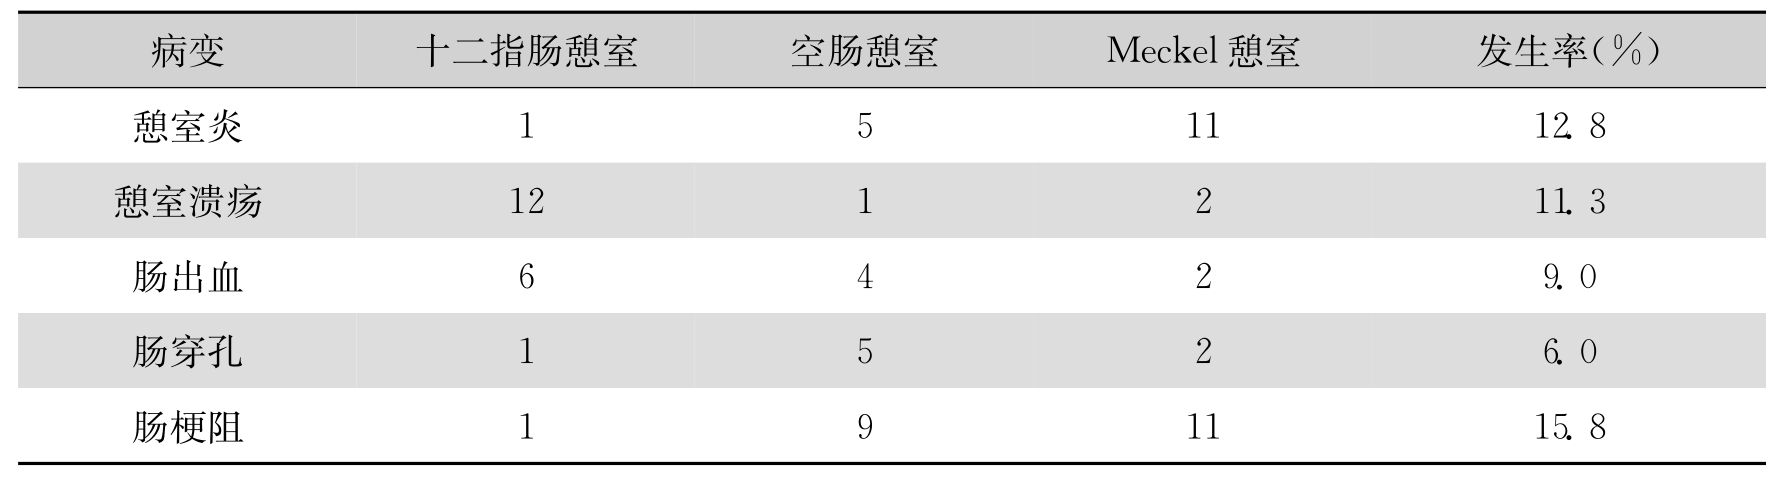
\includegraphics[width=5.91667in,height=1.59375in]{./images/Image00149.jpg}
\end{table}

\subsubsection{八、慢性非特异性十二指肠炎}

有些慢性非特异性十二指肠炎(包括Crohn病或白塞病十二指肠病变),患者主诉上腹部疼痛,进食后或应用制酸剂后缓解,其节律性与周期性也与溃疡病相似,且约1/3病例有上消化道出血,而呕血较为多见。应用胃镜或十二指肠镜是首选的辅助检查手段,内镜下可观察到十二指肠黏膜充血、水肿与肥厚性改变,并可作黏膜活检协助诊断。X线钡餐检查也有一定的诊断参考价值,X线钡餐检查无溃疡龛影,而常发现十二指肠有刺激性改变、痉挛、蠕动过快、黏膜皱襞粗乱或不规则,结合临床情况支持非特异性十二指肠炎的诊断;有人提到由于十二指肠黏膜疣样增生引起的息肉样X线征象,可能是本病较有特异性的表现。

\subsubsection{九、良性十二指肠梗阻}

良性十二指肠梗阻(良性十二指肠壅积症)临床上少见,多发生于瘦长体型的年轻女性。临床上突出的表现是食后上腹部饱胀与不适感或轻度钝痛感,恶心,嗳气,呕吐;呕吐物含有胆汁及隔餐食物。呕吐常于食后2~3小时或夜间发作:患者进食后站立或坐位易诱发呕吐,采取俯卧位或右侧卧位时可使症状缓解。发作时上腹部可见蠕动波,偶可触到扩张的十二指肠。引起慢性十二指肠壅滞的原因颇多,主要是:①肠系膜上动脉分出部位过低,多长、过短;②肠系膜上动脉和腹主动脉之间的角度狭窄;③腹腔脏器粘连牵拉肠系膜上动脉;④内脏下垂牵拉肠系膜;⑤其他因素:先天性异常或畸形,胰或十二指肠肿瘤等。X线钡餐检查可确定本症的诊断,可见胃及十二指肠扩张,幽门通畅无阻,但钡剂不易通至空肠;采俯卧位透视时则钡剂较易排出。

\subsubsection{十、十二指肠结核}

十二指肠结核罕见,大多发生在球部与球后段,也可发生于降段,前者是由胃结核直接蔓延而来,后者可能是泛发性肠结核的一部分,也可单独发病;患者多为20~40岁的青壮年女性,临床表现与胃结核相似。如有大量肉芽组织增生,可阻塞肠腔,临床表现类似幽门梗阻。应用胃镜或十二指肠镜结合组织病理学活检是首选的辅助检查手段;X线钡餐检查对诊断有一定帮助,部分患者最后往往须依靠手术探查及冰冻切片方能确诊。

\subsubsection{十一、原发性十二指肠癌}

原发性十二指肠癌少见,80\%以上发生于壶腹周围及其上方。本病多发生于老年人,但中壮年也可罹患。临床症状可与溃疡病相似,出现慢性上腹痛、上消化道出血或梗阻等症状,但此病有以下特点:经内科积极治疗,大便潜血仍持续阳性;X线钡餐检查显示十二指肠降段或水平段有狭窄、充盈缺损、龛影、黏膜破坏等病变。胃镜或十二指肠镜结合组织病理学活检可确诊。鉴别诊断上须注意与十二指肠结核、憩室及环状胰等相区别。

国内报道原发性十二指肠恶性肿瘤18例中,腺癌16例、平滑肌肉瘤2例。最常见的症状为腹痛(17/18例),十二指肠恶性肿瘤虽少见,但占小肠恶性肿瘤的25\%~45\%,故值得重视。早期表现隐袭,无特征性症状。主要症状为与饮食无关且变化无常的上腹隐痛、体重下降与贫血。肿瘤最多位于降段,X线钡餐与胃十二指肠镜检查均能发现。

\subsection{81.3 胰腺疾病}

\subsubsection{一、慢性胰腺炎}

如患者有与进食有关的、反复发作的上腹痛,以及发热、恶心、呕吐等症状,应注意慢性胰腺炎的可能性,特别是有急性胰腺炎病史者。临床上诊断本病较少,也可能由于目前诊疗手段的限制,造成部分患者出现漏诊。发病多在20~50岁之间,男性多于女性。其病因也较复杂,以胆道疾病(包括胆道蛔虫病)、胰管阻塞、感染、饮酒等较为多见。患者大多数经年反复发作,每次发作均较前一次加重。腹痛及进行性体重下降是慢性胰腺炎的主要临床表现,疼痛多位于左上腹,可呈间歇性或持续性。疼痛部位以中上腹部为多见,其次是心窝部、右上腹部,可放射至腰背部与肩部,疼痛多为阵发性绞痛,少数为钝痛或胀痛。发作持续时间数小时至2~3天不等。饭后疼痛加剧。部分患者可能同时出现腹部包块、腹水、腹泻、黄疸等,黄疸往往在腹痛发作后2~3天出现。体格检查可发现不同程度的上腹部压痛、腹肌紧张,有时可触及肿块。发作期间血象白细胞增多,部分病例血清及尿淀粉酶增高与一过性血糖升高,葡萄糖耐量试验可呈糖尿病曲线。国内彭丽华等报道39例慢性胰腺炎患者,男27例,女12例,男女性别比例为2.25∶1;年龄为3~71岁,平均45.7岁。病程1个月至14年,平均33.9个月。对39例患者的病因分析发现,酒精性占23.1\%,平均饮酒时间(18.3±9.0)年,平均每日饮酒量(151.6±83.9)g;胆源性占46.1\%;特发性占28.2\%;其他类型占2.6\%。临床表现:腹痛占84.4\%,黄疸占12.8\%,便次增多、脂肪泻占12.8\%,体重下降占53.8\%,体重平均下降(12.1±6.7)kg。并发症:胰腺假性囊肿形成(20.5\%)、胆道梗阻(12.8\%)、胰腺癌(2.6\%)、糖尿病(17.9\%)。在缓解期患者可无症状,或有一般消化不良现象。有人认为急性腹痛发作后缓解期间,有左肋弓下深部压痛和两侧肋脊角压痛,往往提示慢性胰腺炎的可能性。脂肪泻、肉质泻、糖尿、体重减轻和营养不良,可出现于晚期病例。

X线腹部平片检查可发现胰腺结石及胰钙化阴影(最常位于第1~2腰椎的右侧);胃肠钡餐X线检查在部分病例可发现邻近器官因慢性胰腺炎症而造成压迫、移位、变形、梗阻或小肠运动功能不良。B超可显示胰腺肿大。近年来,超声内镜作为一种无创性的检查方法,可借助探头透过胃或十二指肠壁对胰腺进行超声探查以获取影像学资料,对胰腺周围结构及大血管的影响也能作出准确的判断,随着高新技术的不断发展,已能把常规的超声探头制作成直径仅1.8~2.0mm的微探头,使胰、胆管内超声(IDUS)检查成为可能。诸琦等报道IDUS对慢性胰腺炎的诊断率为85.7\%,国外文献报道可达95.5\%。

在胰腺外分泌功能试验方面,较有意义的有以下几种:

1.胰功定(BT-PABA)试验对胰腺癌和慢性胰腺炎的敏感性为70\%~87.5\%,特异性为85\%~90.9\%。此法简便,且易为患者所接受。

2.血清胰多肽测定试验餐对慢性胰腺炎的敏感性为85\%,特异性为100\%,均高于胰功定试验。

3.Lundh试验对胰腺癌及慢性胰腺炎的敏感性分别为78\%和83\%~90\%,是一项简便而有效的胰腺外分泌功能试验。

4.胰泌素(secretin)兴奋试验对诊断慢性胰腺疾病,敏感性为75\%~90\%,特异性为90\%。此法需时较久,较不易被患者所接受。

5.放射性核素碘-三油酸甘油酯试验有助于慢性胰腺功能不全的诊断。

慢性胰腺炎的诊断可根据患者的上述临床表现以及下列条件的任何一项而确定之:

(1)慢性胰腺炎组织病理学依据是诊断慢性胰腺炎最有力依据,也是诊断早期或不典型慢性胰腺炎最有力的依据,既往由于获取胰腺组织较困难,有关慢性胰腺炎组织活检尚不能成为常规检查项目,近年来由于开展B超引导下胰腺组织活体检查,对慢性胰腺炎的诊断和治疗将会有更深入地了解。

(2)X线腹部平片检查可发现胰腺结石及胰钙化阴影或胆总管、胰导管逆行造影(ERCP)提示胰管的局限性扩张或狭窄、变形以及假囊肿形成等,应用ERCP对诊断慢性胰腺炎甚有帮助,成功率80\%。但ERCP为侵入性检查法,且可能诱发炎症急性发作,故只在其他方法未能确诊时才考虑应用。

(3)胰腺外分泌功能检测显示有胰腺外分泌功能障碍。

(4)两次以上的上腹痛发作,发作时伴有显著的血清或尿淀粉酶增高(索氏法500U以上)。

(5)血清与尿淀粉酶在发作时虽无明显增高或不增高,但具有下列一种或一种以上的表现者:①胰泌素兴奋试验阳性,并已排除胆道疾病者;②X线腹部平片发现胰腺有钙化阴影或胰腺结石;③胰功定试验、Lundh试验餐、血清胰多肽测定或碘-三油酸甘油酯试验阳性;④其他:如CT、MRCP等对慢性胰腺炎的诊断也有一定的帮助。

慢性胰腺炎与慢性胆道炎症的鉴别有时困难,如患者有上述的诊断条件,而过去无胆绞痛史,X线检查又无胆道结石与胆道炎症征象,则可除外慢性胆道炎症。另一方面,胆囊炎、胆石症并发慢性胰腺炎者也不少见,因此既往急性胰腺炎病史对慢性胰腺炎的诊断有重要意义。

\subsubsection{二、胰腺癌、壶腹周围癌}

凡40岁以上的患者有顽固的上腹痛、厌食和进行性体重减轻等症状时,应注意胰腺癌或壶腹周围癌的可能性。发病年龄多在40~60岁,但30~40岁者也非太少。胰头、胰体与胰尾癌的临床表现有明显区别。黄疸和可触及的胆囊肿大是胰头癌的主要体征,未侵犯胰头的胰体、胰尾癌一般无此特征。

不论胰头癌或壶腹周围癌,腹痛是患者初诊时最常见的主诉,而胰体或胰尾部癌多于胰头癌。腹痛部位最多在中上腹,其次为右上腹,少数于左上腹。多为慢性持续性钝痛,有时呈阵发性剧痛,常放射至腰背部,有时也可放射至右肩部及前胸。疼痛于仰卧时出现或加剧,而前倾坐位或俯卧时可减轻或缓解,这是胰体癌常见的特征。有些早期病例可在左上腹出现短暂的局限性血管杂音,是由于胰体、胰尾癌压迫腹腔动脉的分支(尤其是脾动脉)所引起。结合原因未明的上腹痛,此病征有提示胰体、尾癌早期诊断的意义。国内成文武等总结202例胰腺癌患者的临床特点,发现202例胰腺癌患者,其中男141例,女61例,男女之比2.31∶1。年龄27~84岁,平均56.2岁,>45岁171例(84.65\%)。以胰头癌多见(55.45\%),胰体癌(23.76\%)和胰尾癌(20.79\%)发病率大致相等。临床主要症状与体征:疼痛(47.50\%),疼痛部位见表\ref{tab26-2};其次为消瘦(32.67\%)和黄疸(32.18\%),此外尚有食欲减退、腹胀、腹部不适等症状。

曾有作者对提高胰腺癌早期诊断水平,作出以下建议:40岁以上有下列情况之一者应做有关的检查:①不明原因的上腹痛;②难以解释的体重下降(>10\%);③突发性糖尿病,无肥胖及糖尿病家族史;④难以解释的胰腺炎反复发作。

怀疑胰腺癌的患者,宜选下列实验室或辅助检查,进一步明确诊断:初选B超,诊断的灵敏性与特异性约80\%,对直径≤2.0cm肿瘤诊断较难。螺旋CT双期快速连续扫描可检出直径0.5~1.0cm的肿瘤。B超联合CT灵敏度达到96.8\%。MRI诊断胰腺癌的价值与螺旋CT相似。B超、CT仍未确诊者,应选用ERCP或超声内镜(EUS)检查。EUS可检出直径≤10cm的胰腺癌。近年来,正电子发射体层扫描(PET)也应用于胰腺癌的诊断,尤其是有助于胰腺癌与胰腺良性肿瘤的鉴别。肿瘤标志物如CEA、CA19-9、CA50、C242、CA125等,灵敏性仅27\%~70\%,早期诊断价值有限,主要用于了解病情及术后复发的随访监测。B超或CT引导下经皮细针穿刺(FNA)细胞学诊断,在一组44例早期胰腺癌诊断中,灵敏度92\%,特异性100\%。文献报道,胰腺癌患者血清CA19-9、CA50、CA125、癌胚抗原(CEA)、碱性磷酸酶(ALP)、乳酸脱氢酶(LDH)、甲胎蛋白(AFP)及谷氨酰转肽酶(GGT)的阳性率分别为75.4\%、57.1\%、50\%、38.9\%、56.4\%、35.4\%、3.36\%及58.8\%。B超符合率88.57\%,CT符合率86.81\%,细胞学符合率94.87\%。

\subsubsection{三、胰腺结核}

胰腺结核十分少见,患者通常为青壮年人,一般由腹膜结核蔓延所致。主要临床表现是结核病的全身症状和慢性上腹痛,有时放射至腰背部,多呈胀痛,饭后最为明显,剧痛时弯腰曲背可使症状减轻。结核病患者如有未明原因的慢性上腹痛,脐周附近深部触及实质性包块,宜考虑此病的可能。与慢性胰腺炎不同,血清淀粉酶不增高,也无恶心与呕吐。X线钡餐检查可见十二指肠曲增宽与邻近器官移位。国内报告2例均经剖腹探查而确诊。经积极抗结核治疗后腹痛逐渐缓解,包块缩小至未能触及。

\subsubsection{四、异位胰}

异位胰又名副胰或迷走胰,临床上并非过于少见。这是一种先天性异常,大多数位于胃、十二指肠和空肠,只部分有症状,症状与异位胰所在的部位有关。年龄在13~67岁之间,平均年龄为37.4岁。有临床症状者18例。4例行胃镜下电凝切除;23例剖腹手术切除,其中3例术前确诊。异位胰腺分布部位:胃9例,十二指肠3例,空回肠14例,胆囊1例。胃异位胰最多位于胃幽门部及幽门窦部,多数有上腹部疼痛、不适感与呕吐,表现为溃疡病或幽门梗阻的症状,也可引起大出血,有的病例可误诊为胃痛。十二指肠异位胰引起症状的少见,但也可引起十二指肠溃疡、壅积、出血等并发症。空肠异位胰发生症状的不多,有时也可引起肠出血。以前异位胰须经手术切除标本病理组织标本方能确诊。近年来超声内镜(EUS)有助于异位胰腺的检出和判断;内镜下黏膜下剥离术(ESD)开展,为切除胃内异位胰腺的诊断提供方便。

\subsubsection{五、胰管结石}

胰管结石较少见,随着超声内镜(EUS)和ERCP检查的开展,其检出率有所增加。胰管结石的病因以酗酒为多,其次为胆道疾病、复发性胰腺炎、遗传因素、甲状旁腺功能亢进症等。本病最常见的症状为左上腹痛,呈持续性钝痛或发作性绞痛。其次为腹泻、消瘦及糖代谢异常。40\%患者有胰腺外分泌功能减退。确诊主要依靠X线平片检查。初期结石成分以蛋白质为主,X线检查常呈阴性,诊断须靠超声内镜(EUS)和ERCP检查。结石60\%发生于胰头部,27\%发生于胰体部,其余发生于主胰管尾部和副胰管等处。据报告胰腺结石并发胰腺癌发生率为3.6\%~25\%,故胰腺结石一旦确诊,须注意随诊,如近期症状加重,应考虑癌变可能。国内一组资料显示,癌变率为7.1\%。

\subsection{81.4 空、回肠憩室与憩室炎}

空、回肠憩室既往认为少见,近年来,由于双气囊小肠镜、胶囊内镜的开展,结合X线全消化道气钡双重造影,空、回肠憩室与憩室炎检出率有所上升,可分为先天性与后天性两型,而以后者为多见。多位于空肠上段,发病男多于女。先天型位于肠系膜附着部以外的肠壁,常孤立存在。后天性沿肠系膜边缘,血管经其底部,无正常肌层,因此为假性憩室,黏膜糜烂时可引起出血。患者发病年龄多在40岁以上,均有胃肠道胀气、呃逆、上腹及脐周围疼痛。少数有呕吐、腹泻、营养不良与出血,后者常引起贫血。症状的发生可能由于食物残渣潴留于憩室中,助长某些致病性细菌的繁殖,引起炎症、糜烂、溃疡形成,可并发出血甚至穿孔。

国内另有一组119例小肠憩室报告,便血或潜血阳性51例,上腹胀痛、不适43例,嗳气反酸16例,腹部包块5例,发热7例,肠穿孔5例,肠梗阻3例。憩室的部位位于十二指肠降部72例,十二指肠水平部7例;空肠10例,回肠9例,小肠多发憩室7例,Meckel憩室7例,结肠7例;十二指肠憩室合并食管憩室4例,合并胃部憩室3例。憩室伴肠内瘘3例。有3例在行其他手术时偶然发现。

\subsection{81.5 原发性小肠肿瘤}

既往由于受到检查手段的限制,原发性小肠肿瘤的检出率不高,临床上漏诊、误诊率较高。近年来由于胶囊内镜、小肠镜等应用,导致小肠肿瘤检出率和诊断率明显升高。根据目前的资料,原发性小肠肿瘤以间质瘤最常见,腹痛和消化道出血是最常见的症状。腹部疼痛多为持续性隐痛,但随病情进展而阵发性加剧。临床上未明原因的不完全性肠梗阻应考虑本病。疼痛部位与病变所在颇有关系。原发性小肠肿瘤的诊断主要依靠消化道造影、内镜、腹部B超、腹部CT或选择性腹腔血管造影检查。近年来开展的胶囊内镜和双气囊小肠镜结合活组织检查可显著提高小肠肿瘤的检出率和诊断准确率。

国内报道一组原发性小肠肿瘤132例,男性73例,女性59例,男女之比1.24∶1。发病年龄11~78岁,中位年龄47岁,40岁以上者占71.6\%。主要临床表现为腹部不适、腹痛87例(65.9\%),消化道出血57例(43.2\%),腹部肿块41例(31.1\%),慢性不全性肠梗阻34例(25.8\%),腹痛、出血、腹块同时出现21例(15.9\%)。其他症状还有黄疸、贫血、纳差、体重下降、发热、腹泻等。另一组报道116例原发性小肠肿瘤的病理学特征,其中良性肿瘤16例,腺癌48例,恶性间质瘤27例,恶性淋巴瘤20例,其他恶性肿瘤5例。

\subsection{81.6 肠系膜淋巴结结核}

肠系膜淋巴结结核是腹腔结核常见类型之一,发病多在儿童期与青少年,但壮年有时也可罹患。此病太多继发于肠结核或血行播散型结核病,故往往与肠结核或(及)结核性腹膜炎并存,以致具有复杂的临床表现。病程通常为慢性,在急性进展时可有较明显的发热与剧烈腹痛。局部症状以不同程度的腹痛为主,可为与饮食无关的泛发性腹痛,往往急骤发作,多位于脐部周围。患者尚伴有乏力、食欲减退、消瘦、发热、盗汗等全身中毒症状。腹泻、腹胀也常见。体检早期常无腹部阳性体征,渐而脐周可触及大小不等、质较硬的互相粘连的淋巴结团块,少移动性,伴有压痛。

凡儿童或青少年有原因未明的上述症状,即使未触及腹部肿块,也应考虑此病的可能性。结核菌素试验强阳性对诊断有帮助。腹部平片发现钙化影像也支持此病的诊断。鉴别诊断上主要须与腹内恶性淋巴瘤相区别,两者临床表现相似。如结核可能性较大,可作诊断性抗结核治疗。如经抗结核治疗一个月以上仍无病情改善,须考虑恶性淋巴瘤或其他恶性肿瘤的可能性,必要时腹腔镜下活检或剖腹探查,取得活组织病理标本以明确诊断。近年来开展的经自然腔道腹腔探查术(NOTES)也可取得活组织病理标本以明确诊断,我院目前已对8例腹痛伴不明原因腹水的患者通过NOTES术活检,取得明确诊断(2例间皮瘤、6例腹膜结核)。

\subsection{81.7 肠系膜动脉硬化}

肠系膜动脉硬化可引起发作性动脉痉挛而出现间歇性上腹部发作性疼痛。患者大都是老年人,同时伴有身体其他脏器动脉硬化征象。但确诊须依靠选择性肠系膜动脉造影术。

\subsection{81.8 腹主动脉瘤}

腹主动脉瘤发病常在中年以上,大多由于动脉硬化,少数因外伤、梅毒等所致。腹痛是主要症状之一,其部位可在上腹、脐周或下腹,疼痛大多为持续性钝痛,常因体位改变而加重或减轻,疼痛常放射至背部。体检多能触及搏动性腹块,听诊常听到滚筒样杂音。有作者认为CT
或MRI是值得推荐的诊断方法,只在CT或MRI未能显示瘤体或疑有主动脉分支闭塞时才应用腹主动脉造影术。

\protect\hypertarget{text00205.html}{}{}

\section{82 慢性左上腹痛}

\subsection{82.1 胰腺疾病}

参见第81.3节。

\subsection{82.2 结肠癌}

参见第82节。

\subsection{82.3 脾(肝)曲综合征}

脾(肝)曲综合征的发病可能精神因素、气候变化、饮食不节、结肠功能紊乱、结肠局部气体引起张力增加,结肠过长或下垂、消化道激素分泌异常等与有关,脾(肝)曲综合征系由于结肠功能紊乱所致的疾病。结肠起始于右下腹的盲肠,向上至右上腹后在肝脏下方,接着向左上腹延伸至脾脏下方,再向下行走。结肠在肝脏下方转折处为结肠肝曲,在脾脏下方转折处为脾曲。如果大量气体积聚在脾曲肠腔内,便可引起左下胸和左上腹胀痛,甚至左腰痛,个别可以发生心前区痛,颇似心绞痛,肠内气体排出后,腹痛、腹胀便可减轻或消失,称为脾曲综合征。如气体积聚在右上腹肝曲,则有右上腹或右下胸痛,易误诊为肝、胆疾病,称为肝曲综合征。肝、脾曲综合征大多数发生在从事脑力劳动的中年人中间。肝曲综合征具体表现为右上腹部胀痛或钝痛不适,伴嗳气,下蹲或弯腰不便现象。脾曲综合征以左上腹胀痛为主,严重时甚至出现阵发性剧痛,常伴有心悸、便秘、呼吸困难现象。肝、脾曲综合征发作时间长短不一,常为半小时到数小时,两种综合征体检时,可分别在左上腹或右上腹叩出鼓音。发作时作X线腹部透视,可见肝曲或脾曲明显胀气,但无液平面。肝、脾综合征腹痛症状明显时,容易误诊为慢性肝炎、慢性胆囊炎、十二指肠溃疡或慢性胰腺炎、脾周围炎、慢性胆囊炎,有的甚至还作了手术。目前一般认为脾(肝)曲综合征是结肠功能紊乱,可归入功能性结肠病(参见第79.5节)

\subsection{82.4 慢性脾周围炎}

慢性脾周围炎常为脾脓肿的并发症,也引起左上腹持续性疼痛,常伴有发热、局部压痛,有时可听到脾区摩擦音。

\protect\hypertarget{text00206.html}{}{}

\section{83 慢性左、右腰腹痛}

\subsection{一、肾下垂与游走肾}

肾下垂与游走肾多发生于瘦长体型的女性,以右侧多见,但也可为双侧性。肾脏能在腹部各方向自由活动者,称为游走肾。肾下垂与游走肾可无症状,但也可出现腰酸背痛、肾区钝痛、牵拉痛甚至绞痛等症状,严重时沿输尿管放射。行走、久立、久坐或劳累可诱发症状或使之加剧。在月经期或便秘时疼痛也加重。仰卧或卧向患侧往往使疼痛减轻或消失,有时卧向健侧也可引起患侧的酸痛,部分病例疼痛部位不在腰部而在上腹或下腹,易误诊为胆道疾病或阑尾炎,但肾下垂与游走肾时常明显触到肾脏,其可触程度在卧位与坐位或站位有显著的差异。并发剧烈腹部或腰部疼痛时,在患侧肋脊角至腹股沟可出现皮肤过敏区,与胆道疾病及阑尾炎有鉴别诊断意义。B超、CT或MRI检查与X线肾盂造影检查有助于诊断,参见第101节。

\subsection{二、慢性肾盂肾炎与泌尿道结石}

慢性肾盂肾炎与泌尿道结石可反射性引起肠道功能紊乱,而发生脐周阵发性腹痛。这些疾病同时伴有泌尿系统的症状与体征,鉴别诊断多无困难。

\subsection{三、结肠癌}

右侧结肠癌的腹痛常见而出现较早。国内一组62例中,44例(71\%)以右侧腹痛、上腹痛或全腹痛为最初的症状。有腹痛者60例(97\%),其特点是偶发的针刺样痛或钝痛,多能迅速缓解,以后逐渐加重,发作频繁,进而可伴有腹部鼓包、绞痛,饭后1~2小时疼痛加重,排便或排气后暂时好转。而左侧结肠癌较早的症状往往为大便次数增多,带黏液及血。由于癌变多致肠腔狭窄,又因粪便至此多已形成固体,所以进一步较易引起急性、亚急性或慢性肠梗阻,出现便秘、腹胀、腹鸣与肠绞痛等症状。肠绞痛往往是较晚期的表现。确诊主要依靠结肠镜结合肠黏膜活组织病理组织学检查。

\protect\hypertarget{text00207.html}{}{}

\section{84 慢性右下腹痛}

\subsection{一、慢性痢疾}

慢性痢疾包括慢性阿米巴痢疾和细菌性痢疾细菌性痢疾。慢性阿米巴性痢疾较常引起慢性腹痛,尤以右下腹痛,伴慢性腹泻。确诊靠大便或肠道活检组织找到阿米巴滋养体或包囊,参见第76.1.1节。

\subsection{二、慢性阑尾炎}

慢性阑尾炎是临床上较常见的疾病,主要临床表现为右下腹痛,多呈间歇性轻度疼痛、持续性隐痛或不适感,常局限在右下腹,行走过久过急、剧烈运动、长期站立均可诱发或使症状加重,体检发现右下腹阑尾点有压痛。根据上述临床表现与既往急性阑尾炎病史,一般不难作出诊断。不少患者出现上腹部不适感或疼痛、消化不良症状,易与溃疡病及慢性胆道疾病等相混淆;有时引起痉挛性便秘,类似肠易激综合征或功能性腹痛;女性患者有时可被误认为慢性输卵管炎等盆腔炎症。

慢性阑尾炎有下列特点可与上述疾病相鉴别:①大多数患者过去有急性阑尾炎病史;②上腹部疼痛或不适感无节律性、周期性,但可因进食碱性药物或刺激性小的食物而减轻;③直肠指检可发现直肠前壁右侧有轻度压痛,右下腹阑尾压痛点深触诊常有压痛或不适感,服用轻泻剂后可使疼痛暂时缓解;④X线检查可发现阑尾充盈不正常或不显影,最重要的征象是阑尾点压痛,且压痛随阑尾移动而移位。

临床诊断为慢性阑尾炎,伴有右下腹痛与压痛,而手术证明阑尾完全正常者也有之,故不能单纯以此两项局部症状作为诊断依据。明确的急性阑尾炎病史、上述的消化不良症状、阑尾点压痛、直肠指检、X线钡餐检查等全面检查材料,常有助于确定本病的诊断。

\subsection{三、肠结核}

近年来,结核病(包括肠结核)的发生率有所上升。肠结核多见于20~40岁青壮年,可分为溃疡型与增殖型两型,而以前者较为多见。回盲部是肠结核的好发部位。溃疡型肠结核的主要临床症状是腹痛、腹泻,并伴有发热、盗汗、疲乏、消瘦、贫血等全身症状。腹痛多发生于右下腹,脐周次之,也可波及全腹。疼痛多为轻度至中度阵发性绞痛,也可呈持续性隐痛,往往在食后即出现,以致患者有时怕多进饮食,或误认病在胃而不在肠,此现象的发生是由于食物进入胃后,引起胃结肠、胃回肠反射,而致病变肠段痉挛所致,排便后疼痛可缓解。增殖型肠结核由于黏膜下层、浆膜下层都有结核性肉芽组织增生,因而引起肠狭窄,常有低位肠梗阻症状,常在回盲部可触及压痛不显著的中等硬度腹部肿块。溃疡型肠结核时粪便检查可发现结核菌,但由于多伴有开放性肺结核,而肠内又有其他抗酸杆菌,故涂片染色检查意义不大。肠结核与克罗恩病、白塞病等常难于鉴别。本病的诊断主要依靠电子结肠镜结合肠黏膜活检行组织病理检查(结肠镜下见结肠溃疡呈环形溃疡、病灶<4个等有助于肠结核的诊断),X线全消化道钡餐或钡灌肠气钡双重造影检查有一定的诊断参考价值。其他检查,如PPD试验、血清PPD
IgG等检查参考价值有限。在临床诊治可疑患者时,如综合全面检查材料,以结核病可能性较大时,应即作诊断性抗结核治疗。

\subsection{四、阑尾结核}

阑尾结核临床上极少见,约占阑尾切除标本活检的0.5\%。本病好发于青壮年。可区分为:①粟粒型,最少见,为全身性粟粒型结核病或结核性腹膜炎的局部表现;②溃疡型,最多见,易引起继发感染而致壁内脓肿形成或穿孔;③增殖型,少见,阑尾管壁增厚,外观粗大,有时增大呈肿块状,可误诊为恶性肿瘤或右侧卵巢囊肿。

阑尾结核的体征常不一致,大多数为慢性阑尾炎加上结核病的病征。如患者有肺结核或肠结核病史,右下腹经常有微痛及阑尾点压痛,下午体温略高,兼有体重减轻、乏力、盗汗等症状,应考虑本病的可能性。本病在急性发作时很难与慢性阑尾炎急性发作相鉴别。诊断主要依靠手术探查。手术切除是阑尾结核的基本疗法。

\subsection{五、克罗恩病}

克罗恩病(Crohn病)常累及末段回肠及其邻近结肠。多数患者有腹痛,右下腹痛最多见,大多为隐痛、阵发性加重或反复发作(参见第24章)。

\subsection{六、白塞病}

白塞病的肠道表现可类似Crohn病,伴右下腹痛与消化道出血,常常难以鉴别。白塞病是一种全身性、慢性、血管炎性疾病,主要临床表现是复发性口腔溃疡(92\%~100\%)、生殖器溃疡(约75\%)、眼炎(约50\%)及皮肤损害(80\%~98\%),也可累及血管、神经系统、消化道、关节、肾脏和肺脏等脏器。患者以青壮年为主,30岁左右发病最多,女性稍多于男性。消化道损害发生率约为10\%~50\%,常表现为单发或多发性溃疡,从口腔到肛门均可累及,以回盲部多见。本病临床表现为上腹部饱胀不适、嗳气、吞咽困难、中下腹疼痛、腹泻、黑便及便秘等,严重者可合并穿孔或大出血,在内镜下和组织病理学上无法与Crohn病肠道病变鉴别。诊断标准多采用国际白塞病研究组1989年制定的标准:①复发性口腔溃疡(1年内发作3次或以上);②反复外阴部溃疡;③眼部病变(葡萄膜炎、玻璃体病变及视网膜病变);④皮肤病变(结节样红斑、假性毛囊炎、丘疹性脓疱及痤疮样结节等);⑤针刺试验阳性。复发性口腔溃疡并有其他4项中的2项,排除其他疾病可确诊。值得注意的是,目前临床上上述标准不符合大多数病例的诊断。

\subsection{七、盲肠癌}

盲肠癌在临床上少见,发病年龄多见于50岁以上,临床特点是病程短,进展快,在症状出现后一般即不再缓解,右下腹块的阳性率高,出现也较早。老年患者右下腹痛历时数周而不消失;并有质硬的腹部肿块出现,应考虑盲肠癌的可能性。结肠镜结合肠黏膜活组织病理学检查可明确诊断。

\subsection{八、慢性右侧输卵管卵巢炎}

参见第85节的“慢性盆腔炎”。

\protect\hypertarget{text00208.html}{}{}

\section{85 慢性下腹痛}

\subsection{一、慢性膀胱炎}

慢性膀胱炎常有反复发作的下腹部疼痛,伴有尿频、尿急、尿痛、腰骶部痛、脓尿与菌尿,一般诊断不难。此病可能继发于膀胱结石(参见第36章)。

\subsection{二、慢性前列腺炎、精囊炎}

慢性前列腺炎、精囊炎可引起轻度下腹部隐痛,常伴有早泄、遗精或射精痛,小便终末有黏性分泌物,并发急性炎症时分泌物可为血性。直肠指检可发现前列腺增大或缩小变硬,并有触痛,前列腺液或精液常规及病原体检查可协助诊断(参见第36章)。

耻骨骨炎是一种易被误诊为慢性前列腺炎的疾病,有报告一组28例男性患者,以会阴及下腹部疼痛伴尿痛、尿频及尿后睾丸不适为主诉,易误诊为慢性前列腺炎。但患者肛检前列腺正常,尿常规正常,前列腺液脓细胞<10个/HP。诊断须靠骨盆X线平片检查,明确耻骨病变,并与慢性前列腺炎相鉴别。

\subsection{三、慢性盆腔炎}

慢性盆腔炎患者大多有分娩、流产或阴道器械检查的感染史。腹痛位于下腹部,为持续性隐痛,每于经前期加剧,常伴有白带增多、月经异常、痛经、不孕等表现,下腹部常有轻度压痛。附件炎症以右侧为主者须与慢性阑尾炎相鉴别。妇科检查可发现附件增厚与触痛,结合全面检查材料可与慢性阑尾炎及生殖系结核病相鉴别。

\protect\hypertarget{text00209.html}{}{}

\section{86 慢性左下腹痛}

\subsection{一、慢性细菌性痢疾}

慢性细菌性痢疾较常引起左下腹痛,且常为发作性痉挛性痛,伴里急后重与黏液脓血便(参见第76.1.1节)。

\subsection{二、溃疡性结肠炎}

腹痛是溃疡性结肠炎主要症状之一,部位多在左下腹,常为阵发性绞痛,于排便后消退。腹痛在发作期加剧,缓解期仅有轻度不适甚至无痛(参见第76.1.2节)。

\subsection{三、直肠、乙状结肠癌}

直肠、乙状结肠癌早期症状不明显,一般以左下腹部隐痛、消化不良、体重减轻、便秘或腹泻、或大便习惯改变为多见。癌组织破溃则发生便血(参见第69.2节和第69.3节)。

\subsection{四、结肠憩室与憩室炎}

结肠憩室在儿童与青年少见,50岁以后发病率每10年而明显递增。憩室往往为多数性,主要侵犯乙状结肠与降结肠。患者大多无症状,但也可有左下腹胀痛或不适,间歇性腹胀、便秘、腹泻,或便秘与腹泻交替。如憩室发炎可引起左下腹疼痛与压痛、发热、白细胞增多与排便习惯改变,有时可引起大出血。此病的诊断主要依靠钡剂灌肠造影或电子结肠镜检查。

\subsection{五、慢性左侧输卵管、卵巢炎}

参见第85节“慢性盆腔炎”。

\protect\hypertarget{text00210.html}{}{}

\section{87 慢性广泛性与不定位性腹痛}

\subsection{一、结核性腹膜炎}

结核性腹膜炎是常见病之一,可发生于任何年龄,以21~30岁为多见。本病是继发性,原发病灶最多为肠系膜淋巴结结核、肠结核、输卵管结核、肺结核、胸膜结核等。

本病在病理学上可区分为渗出型、粘连型与干酪型,干酪型病情较重。本病起病可急可缓,缓起者占大多数。主要症状是发热、腹块、腹痛、腹泻,有时腹泻与便秘相交替。腹痛多呈持续性隐痛或钝痛,粘连型有时可出现剧烈的阵发性绞痛。粘连型由于腹膜发炎与显著增厚,腹部触诊多有柔韧感或搓面团感,以及轻度或中度压痛。约1/3病例有腹水征。必要时腹腔镜下活检或剖腹探查,取得活组织病理标本以明确诊断。近年来开展的经自然腔道腹腔探查术(NOTES)也可取得活组织病理标本以明确诊断,我院目前已对8例腹痛伴不明原因腹水的患者通过NOTES术活检,取得明确诊断(2例间皮瘤、6例腹膜结核)。

\subsection{二、腹型恶性淋巴瘤}

腹部恶性淋巴瘤以发生于小肠者最多,也常引起慢性腹痛,多为钝痛或隐痛。如发生不完全性肠梗阻,则引起阵发性肠绞痛。在腹腔脏器恶性淋巴瘤的进行性病例中,常表现为腹块型或腹水型。本病主要须与癌性腹膜炎及结核性腹膜炎相鉴别,往往须经探查方能明确鉴别。原发性肠恶性淋巴瘤是淋巴结以外的恶性淋巴瘤中最常见的。

\subsection{三、消化道多发性息肉综合征}

近年有作者报道消化道多发性息肉病一组,其中12例有腹痛史、8例有便血史。从3例患者的家系调查中,发现15人患本病,研究材料表明本病有很强的家族聚集和遗传性。12例有结肠息肉者,癌变3例,占25\%。

Peutz-Jeghers综合征即黑色素斑-胃肠息肉病,约40\%有家族史。一组18例中,便血16例,腹痛13例。癌变率2\%~3.8\%,可引起肠套叠、肠梗阻等并发症。

Cronkhite-Canada综合征常以慢性隐性腹痛为临床特点。本病特征为:①胃肠道错构瘤息肉病;②有外胚层病变(如脱发、指甲萎缩);③无家族史;④成年发病。

Gardner综合征三联症为:①大肠多发性息肉病;②骨瘤;③皮肤及皮下组织病变。本病为罕见的常染色体显性遗传疾病,肠外病变以皮肤及软组织肿瘤最多见(60\%),骨瘤次之(30\%)。

\subsection{四、腹型肺吸虫病}

据国内报告,腹型肺吸虫病症状以腹痛及压痛为主,有时腹部可触及肿块,可伴有腹泻、便血。当肺吸虫病患者有腹痛、压痛或肿块等症状时,应警惕腹型肺吸虫病的可能。如患者有生食石蟹或蝲蛄史,而无结核病史,有咳嗽及咯铁锈色痰史,痰中发现肺吸虫卵而无结核杆菌,则对此病临床诊断有重要意义。如经肺吸虫病药物治疗无效,可考虑剖腹探查。

\subsection{五、胃肠血吸虫病}

胃肠血吸虫病,最常见是的结肠血吸虫病,尤其是左半结肠更为多见。患者食欲可有不同程度减退,少数有恶心呕吐。半数以上患者病程中有腹痛,腹泻,每日3~5次,严重者可达二三十次。常带黏液和血,重症者粪便呈果酱状。部分患者可有便秘。腹部偶有压痛。少数患者可出现腹水,此可能由于肝、肠急性虫卵肉芽肿的广泛形成,导致肝内窦前高压和肠淋巴渗液增多而漏入腹腔所致。电子肠镜下可见:①急性期:结肠黏膜红肿,外观凹凸不平,部分黏膜表面呈细颗粒状隆起,似砂粒,灰褐色;以后部分黏膜溃破形成浅小的溃疡,大量虫卵由此排入肠腔,此时粪便检查虫卵为阳性。病理活检见肠壁各层均有急性虫卵结节,尤以黏膜下层为明显;结节中央部分坏死,向肠腔溃破形成小溃疡。②慢性期:结肠黏膜和黏膜下层形成假结核结节,最终纤维化,肠壁因纤维组织增生而变厚。肠黏膜萎缩,皱襞变平和消失,且表面粗糙,除有小溃疡外,还常可见黏膜增生形成多发性小息肉;有时可见斑块状分布的浅灰色肠壁不规则增厚区域(为大量钙化的虫卵沉积所致)。病理活检可见各种不同阶段的急性、慢性虫卵结节;晚期,因虫卵死亡或钙化,肠黏膜溃疡已愈合,增厚的肠壁难以使虫卵排出,故粪检虫卵可为阴性。此时,需要作肠黏膜压片或活组织检查才能找到虫卵而确诊。大肠血吸虫病癌变并发率高。有文献报道,经病理检查证实的血吸虫病患者166例中男132例,女34例,男女比约4∶1,平均年龄45.8岁,最大82岁,最小仅8岁,其中<20岁12例,20~39岁48例,40~60
岁71例,>60岁35例。病程3天至3年不等,多数为半年。临床表现主要为:腹泻(6.63\%)、腹痛(37.95\%)、腹痛与腹泻交替进行(3.01\%)、便血(33.73\%)、腹部包块(5.42\%)、食欲下降及消瘦(2.4\%)、排便困难(5.42\%)、呕血黑便(1.80\%)、发热等。病变部位以结肠(21.69\%)、直肠及肛管(32.53\%)、回盲部及阑尾(39.16\%)多见,其他为胃(6.02\%)、十二指肠、空肠、胃周淋巴结及系膜、肝脾、颞叶、附睾等。

\subsection{六、腹膜粘连}

手术后引起的肠粘连甚常见,外伤后或腹膜炎后也常发生肠粘连。粘连程度可轻可重,轻症者可无症状或仅有轻微的腹部不适,重症者可发生机械性肠梗阻。腹膜粘连的腹痛,严重时为绞痛性,多在食后发作,发作时腹部听诊可发现肠鸣音亢进。X线或腹腔镜检查有助于诊断。

\subsection{七、慢性假性肠梗阻}

肠假性梗阻是一种无机械性肠腔阻塞而具有肠梗阻症状和体征的无效性肠推进运动造成的一个临床综合征,可呈急性或慢性起病。发病机制尚未明了。

慢性病例可为原发性或继发性。原发性者又称为慢性特发性假性肠梗阻(CIIP)。继发性者则继发于进行性系统性硬皮病(PSS)、淀粉样变、Chagas病、使用某些药物如氯丙嗪后等。CIIP病程长,亦未发现有基础病,主要临床表现为中、上腹痛,腹胀,体重减轻,便秘或腹泻、呕吐等。体检腹部可见肠型蠕动、肠鸣亢进,也可有肠鸣消失。腹部平片显示小肠及(或)结肠扩张,严重者可见液平面。诊断应首先详细分析病史和症状,排除机械性肠梗阻,密切动态观察,进行一般支持疗法,有基础病或并发症者适当处理。

\subsection{八、腹膜癌}

腹膜癌是继发性,也可引起腹痛,但一般程度较轻(参见第94节)。

\subsection{九、血卟啉病}

血卟啉病也可反复出现腹部疼痛,持续时间由几小时至数天甚至数周不等。间隔期可长可短(参见第79.2节)。

\subsection{十、肠寄生虫病}

钩虫、蛔虫、绦虫、姜片虫、粪类圆线虫、长膜壳绦虫等肠道寄生虫均可引起慢性不定位腹痛,腹痛性质可为隐痛或绞痛;后者由蛔虫性肠梗阻引起。

\subsection{十一、腹型过敏性紫癜}

腹型过敏性紫癜可反复出现不定位的腹部疼痛。

\subsection{十二、内分泌功能紊乱}

垂体前叶功能减退症与慢性肾上腺皮质功能减退症均可出现痉挛性腹痛,提示低血钠与低血糖反应。甲状旁腺功能亢进或减退症也可引起不同程度的痉挛性腹痛,有时与消化性溃疡病腹痛相似,但一般无规律性。

\subsection{十三、系统性肥大细胞增多症}

系统性肥大细胞增多症亦称系统性肥大细胞病,病因不明,国内仅有少数病例报告。组织肥大细胞分布于全身各种组织,故患病时症状繁多。本病主要临床表现为:①皮肤症状:皮肤潮红、色素性荨麻疹等;②消化系症状:恶心、呕吐、腹痛、腹泻等,常伴有肝大;③心血管症状:心动过速、低血压等;④其他症状:发热、头痛、乏力、贫血、抽搐等。反复发作的不明原因腹痛(可蔓延及全腹)提示本病诊断的可能。骨髓呈组织嗜碱性细胞增生,血和尿液组胺浓度明显增高,可确定诊断。尿5-HIAA正常,可除外类癌综合征。

\subsection{十四、结缔组织病}

结节性多动脉炎引起腹痛者常见。国内文献报道系统性红斑狼疮约50\%病例有腹痛,部位大多局限于脐周。

\subsection{十五、Castleman病}

Castleman病是一种临床较为罕见的疾病,极易误诊。组织学特点主要为:血管玻璃体样改变的血管透明型(HV型),以浆细胞增生为主的浆细胞型(PC)型及混合型(Mix型)。主要以间歇性腹痛伴反复不完全性肠梗阻为特点(肠镜检查未发现异常),查体腹部无肿块,仅有压痛。腹腔淋巴结行免疫组化可确诊为Castleman病。

\subsection{十六、功能性胃肠病}

\subsubsection{1.肠易激综合征}

肠易激综合征及功能性腹痛是功能性胃肠病的其中两种类型。肠易激综合征是一组包括腹痛、腹胀、排便习惯和大便形状异常,常伴有黏液便,持续存在或反复发作,而又缺乏形态学和生化学异常者,其发病原因尚未完全明了。病程呈慢性经过,常长期反复发作,但对患者健康情况一般无大影响,与结肠癌症状呈进行性恶化者不同。主要症状是阵发性痉挛性肠绞痛,部位常在左下腹与下腹部,而甚少在脐周。情绪激动、劳累可诱发腹痛发作,排气或排便后症状缓解,腹痛发作时常伴有大便形状或(和)次数的改变,可表现为便秘或腹泻,或便秘与腹泻交替。大便可为稀烂或水样,也可坚硬如羊粪,常附有黏液。体检可触及痉挛的结肠,特别是乙状结肠。大便检查除有黏液外,无脓血或白细胞及其他病理成分。结肠镜检查、X线钡剂灌肠检查正常或仅见局部结肠痉挛而无其他异常。值得注意的是,本病的诊断需先排除其他消化系统和全身器质性疾病所致的这一症状群。

\subsubsection{2.功能性腹痛综合征}

功能性腹痛综合征(functional abdominal pain
syndrome,FAPS)又称慢性特发性腹痛或慢性功能性腹痛,是指持续或频繁发作的下腹痛,病程超过半年,但无胃肠道功能紊乱症状的一组临床症候群。FAPS患者常有抑郁、焦虑等心理障碍、并常伴随躯体其他部位的不适和日常活动受限。FAPS主要表现为起病缓慢、腹痛,腹痛呈持续性或反复发作,不受生理活动影响(如饮食、排便等),有些患者的病史可追溯到儿童时期。多无明显体征,无固定的压痛点。部分患者可伴有心动过速、出汗、血压改变和焦虑抑郁等症状。诊断功能性腹痛必须十分小心通过体检、实验室及器械检查排除器质性疾病,并进行较长时间的临床随访,以免遗漏器质性疾病引起的腹痛。

\protect\hypertarget{text00211.html}{}{}

\section{参考文献}

1.朱砚蕴,等.胃血吸虫病135例分析.中华医学杂志,1986,65:16

2.罗忠芬.慢性胃扭转12例分析.上海医学,1989,12:662

3.史在新.原发性胃淋巴瘤25例临床分析.中华内科杂志,1989,28:616

4.王维东.原发性十二指肠恶性肿瘤.上海医学,1990,13:572

5.徐家裕.Lundh试验的临床应用.中华消化杂志,1981,1:242

6.潘树平.消化道内异位胰12例报告.上海医学,1989,12:605

7.炳生.小肠平滑肌肿瘤.上海医学,1989,12:149

8.鲁重美.原发性肠恶性淋巴瘤------67例临床病理研究.中华内科杂志,1987,26:344

9.江石湖.消化超声内镜的应用.中华消化杂志,1990,18(3):131

10.黄志强.加强对胆囊癌的诊断与治疗.中华外科杂志,1997,35(11):643

11.吴云林.超声胃镜对肥厚胃黏膜性质的诊断.中华消化杂志,1994,14(6):318

12.牟善功,等.327例胃癌前病变胃镜随访报告.中华内科杂志,1994,33(6):406

13.关勋,等.胰腺结核的诊断和治疗.中华结核和呼吸杂志,1998,21(11):689

14.孙亚新,梁燕燕.假瘤型慢性胰腺炎五例.中华内科杂志,1993,92(5):392

15.李北申,等.胰管结石15例报告.中华消化杂志,1992,12(4):238

16.李盟,李庆瑞.成人环状胰腺20例报告.中华消化杂志,1995,15(1):58

17.张兆祥,等.阑尾结核15例临床病理观察.中华结核和呼吸杂志,1996.19(4):236

18.陈祖望,等.CT在腹主动脉瘤的诊断价值.中华心血管杂志,1997,20(6):361

19.梁浩,等.结肠镜检诊断小肠憩室141例资料分析.中华内科杂志,1995,34(9):624

20.何小东,等.119例小肠憩室的临床治疗分析.中国胃肠外科杂志,2000,3(4):245

21.梁浩,等.8例肠型白塞病临床分析.中华消化杂志,1997,17(1):61

22.姜军,等.肠系膜淋巴结结核的诊断和外科治疗.中华结核和呼吸杂志,1998,21(5):273

23.张立力,等.胃肠道多原发恶性肿瘤35例分析.中华内科杂志,1999,38(2):88

24.刘彤,等.116例原发性小肠肿瘤的临床病理分析.中华胃肠外科杂志,2002,5(4):259

25.姜海洋,等.耻骨骨炎------一种易误诊为前列腺炎的疾病.中华外科杂志,1991,29(9):579

26.张月彩,等.18例Peutz-Jeghers综合征临床病理分析.中华消化杂志,1996,16(5):310

27.杨利生,等Cronkhite-Canada综合征.中华消化杂志,1995,15(2):77

28.谷成明,等.Gardner综合征三例.中华消化杂志,1992,12(4):241

29.诸琦,等.胰管内超声在鉴别胰腺癌和慢性胰腺炎中的临床应用价值.中华消化杂志,2000,20:255-257

30.蒋国平,等.原发性小肠肿瘤的诊断(附132例临床分析).实用肿瘤杂志,2000,15(3):203

31.吴小平,等.溃疡性结肠炎398例结肠镜检查分析.中华消化杂志,2002,22(11):673

32.郑家驹,等.克罗恩病的临床多样性.中华消化杂志,2002,22(4):226

33.周宗斌,等.166例血吸虫病例分析.中华消化杂志,2004,24(2):122

34.张帆,姜军,杨新华,等.异位胰腺的诊断和治疗(附27例报告).消化外科,2004,05:31-33

35.张欣,厉有名.235例原发性小肠肿瘤的诊治分析.浙江大学硕士论文(2011)

36.郑树国,王小军.胆囊切除术后综合征.中国实用外科杂志,2008,28(6):510-512

37.DeVault KR.,Castell DO.Updated guidelines for the diagnosis and
treatment of gastroesophageal reflux disease.American Journal of
Gastroenterology,2005,100:190-200

38.中华医学会消化病学分会.慢性胰腺炎诊治指南(2005年,南京).中华内科杂志,2005,44(8):637-638

\protect\hypertarget{text00212.html}{}{}

